\documentclass[a4paper]{article}
\usepackage{geometry}
\geometry{
	a4paper,
	total={170mm,257mm},
	left=27mm,
	right=30mm,
	top=30mm,
	bottom= 30mm
}
\usepackage{tabu}
\usepackage[english]{babel}
\usepackage[utf8]{inputenc}
\usepackage{longtable}
\usepackage{amsmath}
\usepackage{graphicx}
\usepackage{enumitem}
\usepackage[colorinlistoftodos]{todonotes}
\usepackage{tikz}
\newcommand*\circled[1]{\tikz[baseline=(char.base)]{
		\node[shape=circle,draw,inner sep=0.5pt] (char) {#1};}}
\usetikzlibrary{fit,positioning}
\usepackage{authblk}
\usepackage{natbib}
\usepackage[algo2e]{algorithm2e}
\usepackage{algorithmic}  
\usepackage{algorithm}
\usepackage{comment}
\usepackage{array}% http://ctan.org/pkg/array
\makeatletter
\g@addto@macro{\endtabular}{\rowfont{}}% Clear row font
\makeatother
\newcommand{\rowfonttype}{}% Current row font
\newcommand{\rowfont}[1]{% Set current row font
	\gdef\rowfonttype{#1}#1%
}
\newcolumntype{L}{>{\rowfonttype}l}
\title{Interaction-Partitioned Topic Models (IPTM) \\using a Point Process Approach}
%\author{Bomin Kim}

\author[1]{Bomin Kim}
\author[1]{Bruce Desmarais}
\author[2,3]{Hanna Wallach}
\affil[1]{Pennsylvania State University}
\affil[2]{Microsoft Research NYC}
\affil[3]{University of Massachusetts Amherst}

\begin{document}
\maketitle
\section{Ideas}
Current CPME model does not involve any of temporal component, which plays a key role in email interactions. Intuitively, past interaction behaviors significantly influence future ones; for example, if an actor $i$ sent an email to actor $j$, then $j$ is highly likely to send an email back to $i$ as a response (i.e. reciprocity). Moreover, the recency and frequency of past interactions can also be considered to effectively predict future interactions. Thus, as an exploratory data analysis, point process model for directional interaction is applied to the North Carolina email data. Starting from the existing framework focused on the analysis of content-partitioned subnetworks, I would suggest an extended approach to analyze the data using the timestamps in the email, aiming to develop a joint dynamic or longitudinal model of text-valued ties.\\ \newline
 CPME model is a Bayesian framework using two well-known methods: Latent Dirichlet Allocation (LDA) and Latent Space Model (LSM). Basically, existence of edge depends on topic assignment $k$ (LDA) and its corresponding interaction pattern c. Each topic $k=1,…,K$ has one interaction pattern c=1,…,C, and each interaction pattern posits unique latent space (LSM), thus generating $A\times A$ matrix of probabilities $P^{(c)}$ that a message author
a will include recipient $r$ on the message, given that it is about
a topic in cluster $c$.  Incorporating point process approach, now assume that under each interaction pattern, we have $A\times A$ matrix of stochastic intensities at time $t$, $\boldsymbol{\lambda}^{(c)}(t)$, which depend on the history of interaction between the sender and receiver. We will refer this as  interaction-partitioned topic models (IPTM). 
\section{IPTM Model}
In this section, we introduce multiplicative Cox regression model for the edge formation process in a longitudinal communication network. For concreteness, we frame our discussion of this model in terms of email data, although it is generally applicable to any similarly-structured communication data.
\subsection{Point Process Framework}
A single email, indexed by $d$, is represented by a set of tokens $w^{(d)} = \{w^{(d)}_m \}_{m=1}^{M^{(d)}}$ that comprise the
text of that email, an integer $i^{(d)} \in \{1,...,A\}$ indicating the identity of that email’s sender, an integer $j^{(d)} \in \{1,...,A\}$ indicating the identity of that email’s receiver, and an integer $t^{(d)} \in [0, T]$ indicating the (unix time-based) timestamp of that email. To capture the relationship between the interaction patterns expressed in an email and that email’s recipients, documents that share the interaction pattern $c$ are associated with an $A\times A$ matrix of $\boldsymbol{\lambda}^{(c)}(t)=\{\{\lambda^{(c)}_{ij}(t)\}_{i=1}^{A}\}_{j=1}^{A}$, the stochastic intensity where $\lambda^{(c)}_{ij}(t)dt$=P\{for interaction pattern $c$, $i\rightarrow j$ occurs in time interval $[t, t+dt)\}$. We will model the counting process $\mathbf{N}^{(d|c)}(t)$ through $\boldsymbol{\lambda}^{(c)}(t)$ using a version of the Cox proportional intensity model, where $N_{ij}^{(d|c)}(t)$ denotes the number of edges (emails) for document $d$ from actor $i$ to actor $j$ up to time $t$ (from the starting point 0) given that the document corresponds to interaction pattern $c$. Since this counting proess $\mathbf{N}$ is document-based, each element is either 0 or 1, and only one element of the matrix is 1 while all the rests are 0 (assuming no multicast). \\ \newline Combining the individual counting processes of all potential edges,  $\mathbf{N}^{(d|c)}(t)$ is the multivariate counting process with $\mathbf{N}^{(d|c)}(t)=(N^{(d|c)}_{ij}(t): i, j \in {1, ..., A}, i \neq j)$. Here we make no assumption about the independence of individual edge counting process. As in \cite{Vu2011}, we model the multivariate counting process via Doob-Meyer decomposition:
\begin{equation}
\mathbf{N}^{(d|c)}(t)=\int_0^t\boldsymbol{\lambda}^{(c)}(s)ds + \mathbf{M}(t)
\end{equation}
where essentially $\boldsymbol{\lambda}^{(c)}(t)$ and $\mathbf{M}(t)$ may be viewed as the (deterministic) signal and (martingale) noise, respectively.\\ \newline
Following the multiplicative Cox model of the intensity process $\boldsymbol{\lambda}^{(c)}(t)$ given $\boldsymbol{H}_{t-}$, the entire past of the network up to but not including time $t$, we consider for each potential directed edge $(i, j)$ the intensity forms:
\begin{equation}
\lambda^{(c)}_{ij}(t|\boldsymbol{H}_{t-})=\lambda_0\cdot \mbox{exp}\Big\{\boldsymbol{\beta}^{(c)T}\boldsymbol{x}_t(i, j)\Big\}\cdot 1\{j \in \mathcal{A}^{(c)}\}
\end{equation}
where $\lambda_0$ is the common baseline hazards for the overall interaction, $\boldsymbol{\beta}^{(c)}$ is an unknown vector of coefficients in $\boldsymbol{R}^{p}$, $\boldsymbol{x}_t(i, j)$ is a vector of $p$ statistics for directed edge $(i, j)$ constructed based on
$\boldsymbol{H}_{t-}$, and $\mathcal{A}^{(c)}$ is the predictable receiver set of sender $i$ corresponding to the interaction pattern $c$ within the set of all possible actors $\mathcal{A}$. Equivalently, by fixing $\lambda_0=1$, we can rewrite (2): 
\begin{equation}
\lambda^{(c)}_{ij}(t|\boldsymbol{H}_{t-})= \mbox{exp}\Big\{\boldsymbol{\beta}^{(c)T}\boldsymbol{x}^*_t(i, j)\Big\}\cdot 1\{j \in \mathcal{A}^{(c)}\}
\end{equation}
where the first element of $\boldsymbol{\beta}^{(c)}$ corresponds to the deviation from $\lambda_0$, by setting $\boldsymbol{x}^*_t(i, j)=(\boldsymbol{1}, \boldsymbol{x}_t(i, j))$.\\ \newline
Based on the framework illustrated so far, the likelihood we will use for inference procedure is that of  \cite{PerryWolfe2012}. For each type of interaction pattern $c=1,...,C$, estimation for $\boldsymbol{\beta}^{(c)}$ proceeds by maximizing the so-called partial likelihood of \cite{cox1992regression}: 
\begin{equation}
PL_t(\boldsymbol{\beta}^{(c)})=\prod_{d: c^{(d)}=c} \frac{\mbox{exp}\{\boldsymbol{\beta}^{(c)T}x_{t^{(d)}}(i^{(d)}, j^{(d)})\}}{\sum_{j\in \mathcal{A}^{(c)}} \mbox{exp}\{\boldsymbol{\beta}^{(c)T}x_{t^{(d)}}(i^{(d)}, j)\}},
\end{equation}
where $t^{(d)}$, $i^{(d)}$, and $j^{(d)}$ are the time, sender, and receiver
	of the $d$th document. For computational efficiency, we will use the log-partial likelihood:
\begin{equation}
\mbox{log}PL_t(\boldsymbol{\beta}^{(c)})=\sum_{d: c^{(d)}=c} \Big\{\boldsymbol{\beta}^{(c)T}x_{t^{(d)}}(i^{(d)}, j^{(d)})-\mbox{log}\big[\sum_{j\in \mathcal{A}^{(c)}}\mbox{exp}\{\boldsymbol{\beta}^{(c)T}x_{t^{(d)}}(i^{(d)}, j)\}\big]\Big\}.
\end{equation}
\subsection{Generative Process}
The generative process of this model follows the topic model (LDA) of \cite{Blei2003} and the author-topic model of \cite{rosen2004author}. Same as LDA, documents are represented as random mixtures over latent topics, where each topic is characterized by a distribution over words. However, one crucial difference is that each document is connected to one type of interaction pattern, and the topic distributions vary depending on the assigned interaction pattern. \\ \newline Conditioned on the interaction pattern and their distributions over topics, the process by which a document is generated can be summarized as follows: first, an interaction pattern is chosen by multinomial for each document; next, a topic is sampled for each word from the distribution over topics associated with the interaction pattern of the document; finally, words themselves are sampled from the distribution over words associated with each topic. At the same time, the unique sender-recipient pair of the document is determined by the rate of intensities associated with the interaction pattern and history of interactions until the time the document is written. Below are the detailed generative process for each document in a corpus $D$ and its plate notation (Figure 1), and Table 1 summarizes the notations used in this paper:
\begin{itemize}
	\item[1.] {$\boldsymbol{\phi}^{(k)} \sim \mbox{Dir}(\delta, \bf n)$} \textbf{[See Algorithm 1]}\\
	- A “topic” $k$ is characterized by a discrete distribution over $V$ word types with probability vector $\phi^{(k)}$. A symmetric Dirichlet prior with concentration parameter $\delta$ is placed.
\item[2.] For each of the $C$ interaction patterns \textbf{[See Algorithm 2]}:
\begin{itemize}
	\item[(a)] $\boldsymbol{\beta}^{(c)}\sim \mbox{Normal}(\textbf{0}, \sigma^2I_P)$\\ 
	- The vector of coefficients depends on the interaction pattern $c$. This means that there is variation in the degree of influence from the network statistics $\boldsymbol{x}_t(i, j)$ that rely on the history of interactions.
	\item[(b)] Using $\boldsymbol{\beta}^{(c)}$ in (a), update $\boldsymbol{\lambda}^{(c)}(t)$\\
	- We use the equation $\lambda^{(c)}_{ij}(t)= \mbox{exp}\Big\{\boldsymbol{\beta}^{(c)T}\boldsymbol{x}^*_t(i, j)\Big\}\cdot 1\{j \in \mathcal{A}^{(c)}\}$ for all $i \in \mathcal{A}, j \in \mathcal{A}, i\neq j$.
	\item[(c)] $\boldsymbol{\theta}^{(c)}\sim \mbox{Dir}(\alpha, \textbf{m})$\\
	- Each email has a discrete distribution over topics $\boldsymbol{\theta}^{(c)}$, since the topic proportions for documents in the same cluster are drawn from the same distribution. The Dirichlet parameters $\alpha$ and $\textbf{m}$ may or may not vary by interaction patterns.
\end{itemize}
\item[3.] For each of the $D$ documents \textbf{[See Algorithm 3]}:
\begin{itemize}
	\item[(a)] $c^{(d)}\sim \mbox{Multinomial}(\boldsymbol{\gamma})$\\
	- Each document $d$ is associated with one ``interaction pattern" among $C$ different types, with parameter $\boldsymbol{\gamma}$. Here, we assign the prior for the multinomial parameter $\boldsymbol{\gamma} \sim \mbox{Dir}({\eta}, \boldsymbol{l})$
	\item[(b)] $\mathbf{N}^{(d|c^{(d)})}(t^{(d)}) \sim \mbox{CP}(\boldsymbol{\lambda}^{(c^{(d)})}(t^{(d)}))$\\
	- The actual update of the counting process $\mathbf{N}^{(d|c^{(d)})}(t)$ of the email $d$ is  $N^{(d|c^{(d)})}_{i^{(d)}j^{(d)}}(t^{(d)})=1$ and the rest $N^{(d|c^{(d)})}_{(i, j) \neq (i^{(d)}, j^{(d)})}(t^{(d)})=0$.
\end{itemize}
\item[4.] For each of the $M$ words \textbf{[See Algorithm 4]}:
\begin{itemize}
	\item[(a)] $z_m^{(d)} \sim \mbox{Multinomial}(\boldsymbol{\theta}^{(c^{(d)})})$
\item[(b)] $w_m^{(d)} \sim\mbox{Multinomial} (\phi^{(z_m^{(d)})})$
\end{itemize}
\end{itemize} 
 \begin{algorithm}[H]
 	\SetAlgoLined
 	\caption{Topic Word Distributions}
 	\For{k=1 to K}{
 		draw $\boldsymbol{\phi}^{(k)}$ $\sim$ Dir($\delta, \bf n$)
 	}
 \end{algorithm}
 \begin{algorithm}[H]
 	\SetAlgoLined
 	\caption{Interaction Patterns}
 	\For{c=1 to C}{
 		draw $\boldsymbol{\beta}^{(c)}\sim \mbox{Normal}(\textbf{0}, \sigma^2I_P)$\\
 	\For{i=1 to A}{
 	\For{j=1 to A}{
 		\If{i $\neq$ j}{ set $\lambda^{(c)}_{ij}(t)= \mbox{exp}\Big\{\boldsymbol{\beta}^{(c)T}\boldsymbol{x}^*_t(i, j)\Big\}\cdot 1\{j \in \mathcal{A}^{(c)}\}$}
 	\Else {set $\lambda^{(c)}_{ij}(t)=0$}
 		}}
 			draw $\boldsymbol{\theta}^{(c)}$ $\sim$ Dir($\alpha, \textbf{m}$)
 	}
 \end{algorithm}
 \begin{algorithm}[H]
 	\SetAlgoLined
 	\caption{Document-Interaction Pattern Assignments}
 	\For{d=1 to D}{
 		draw $c^{(d)}$ $\sim$ Multinomial($\boldsymbol{\gamma}$)\\
 			draw $\mathbf{N}^{(d|c^{(d)})}(t^{(d)}) \sim \mbox{CP}(\boldsymbol{\lambda}^{(c^{(d)})}(t^{(d)}))$
 	}
 \end{algorithm}
 \begin{algorithm}[H]
 	\SetAlgoLined
 	\caption{Tokens}
 	\For{d=1 to $D$}{
 		set ${M}^{(d)}$ = the number of words in document $d$\\
 		\For{m=1 to ${M}^{(d)}$}{
 			draw $z_m^{(d)} \sim \mbox{Multinomial}(\boldsymbol{\theta}^{(c^{(d)})})$\\
 		{draw $w_m^{(d)} \sim\mbox{Multinomial} (\boldsymbol{\phi}^{(z_m^{(d)})})$
 		}}
}
 \end{algorithm}
 \small
 \begin{figure}[ht]
 	\centering
 	\scalebox{1}{ 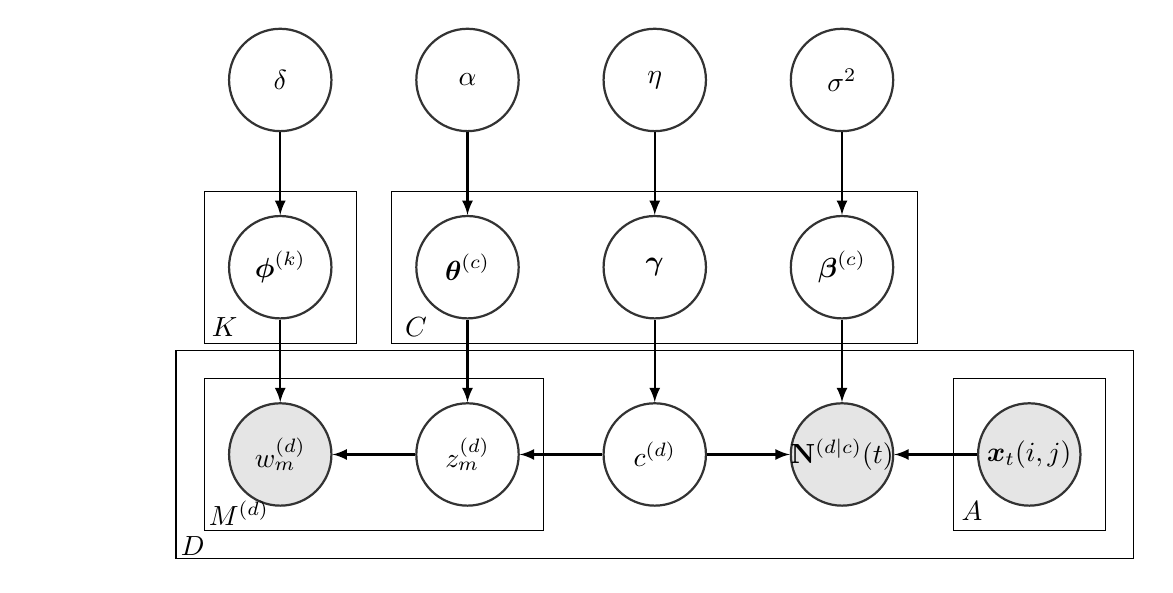
\begin{tikzpicture}
 	\tikzstyle{main}=[circle, minimum size = 13mm, thick, draw =black!80, node distance = 10.5mm]
 	\tikzstyle{connect}=[-latex, thick]
 	\tikzstyle{box}=[rectangle, draw=black!100]
 	\node[main, fill = white!100] (gamma) [label=center:$\boldsymbol{\gamma}$] { };
 	\node[main] (c) [below=of gamma,label=center:$c^{(d)}$] { };
 		\node[main, fill = black!10] (N) [right=of c ,label=center:$\mathbf{N}^{(d|c)}(t)$] { };	
 		\node[main] (z) [left=of c,label=center:$z_m^{(d)}$] {};
 	\node[main, fill = black!10] (w) [left=of z,label=center:$w_m^{(d)}$] { };
 	\node[main] (phi) [above=of w,label=center:$\boldsymbol{\phi}^{(k)}$] { };
 	\node[main] (delta) [above=of phi,label=center:$\delta$] { };
 	 			\node[main] (eta) [above=of gamma,label=center:${\eta}$] { };
\node[main, fill = black!10] (x) [right=of N,label=center:$\boldsymbol{x}_t{(i,j)}$] { };
 	 		 	 						\node[main] (beta) [above=of N ,label=center:$\boldsymbol{\beta}^{(c)}$] { };
 	 		 	 							\node[main] (theta) [above=of z,label=center:$\boldsymbol{\theta}^{(c)}$] { };
 	 		 	 										 	\node[main] (alpha) [above=of theta,label=center:$\alpha$] { };
 	 		 	 						 	 		\node[main] (sigma) [above=of beta,label=center:$\sigma^2$] { };
 	\path (gamma) edge [connect] (c)
 	(z) edge [connect] (w)
 	(theta) edge [connect] (z)
 	(alpha) edge [connect] (theta)
 	(phi) edge [connect] (w)
 	(delta) edge [connect] (phi)
 	(sigma) edge [connect] (beta)
 	(x) edge [connect] (N)
 	(beta) edge [connect] (N)
 	(c) edge [connect] (N)
 	(c) edge [connect] (z)
 		(eta) edge [connect] (gamma);
 			\node[rectangle, inner sep=3mm, fit=  (x),label=below left:$A$, xshift=5mm, yshift=5mm] {};
 			\node[rectangle, inner sep=3mm,draw=black!100, fit= (beta)(theta)] {};
 				\node[rectangle, inner sep=4mm, fit=  (beta)(theta) ,label= below left:$C$, xshift=-17mm, yshift=5.5mm] {};
 	\node[rectangle, inner sep=3mm, draw=black!100, fit= (phi)] {};
 		\node[rectangle, inner sep=3mm, draw=black!100, fit= (x) ] {};
 		\node[rectangle, inner sep=0mm, fit= (phi),label=below left:$K$, xshift=2.5mm, yshift=1.5mm] {};
 	\node[rectangle, inner sep=0mm, fit= (w),label=below left:$M^{(d)}$, xshift=6.5mm, yshift=2mm] {};
 	\node[rectangle, inner sep=3mm,draw=black!100, fit= (w)(z)] {};
 	\node[rectangle, inner sep=4mm, fit= (c) (N) (x) ,label=below left:$D$, xshift=-69mm, yshift=1.5mm] {};
 	\node[rectangle, inner sep=6.6mm, draw=black!100, fit =(c) (z) (w) (N) (x) ] {};
 	\end{tikzpicture}}
 	\caption{Plate notation of IPTM}
 	\label{fig:plate}
 \end{figure}
 \begin{table}[ht]
 	 \centering
\scalebox{0.8}{ 	\begin{tabular}{ |c|c|c|} 
	\hline
 		\hline
 	Authors of the corpus &$\mathcal{A}$ & Set\\
 		\hline
 			Authors of the corpus given interaction pattern $c$ &$\mathcal{A}^{(c)}$ & Set\\
 			\hline
 	Number of authors &$A$ & Scalar \\
 		\hline
 		 	Number of documents &$D$ & Scalar \\
 		 	\hline
 		 	 	Number of words in the $d^{th}$ document &$M^{(d)}$ & Scalar \\
 		 	 	\hline
  	Number of topics & $K$ & Scalar \\
  	\hline
  	  Vocabulary size & $W$ & Scalar \\
  	  	\hline
  	 	Number of interaction patterns &$C$ & Scalar \\
  	 	\hline
  	 		Number of words assigned to interaction pattern and topic&$M^{CK}$ & Scalar \\
  	 		\hline
  	 			Number of words assigned to word and topic&$M^{WK}$ & Scalar \\
  	 			\hline
  	 	Interaction pattern of the $d^{th}$ document&$c^{(d)}$ & Scalar\\
  	 	\hline 
  	 	Time of the $d^{th}$ document&$t^{(d)}$ & Scalar\\
  	 		\hline 
  		Words in the $d^{th}$ document&$\boldsymbol{w}^{(d)}$ & $M^{(d)}$-dimensional vector\\
  		\hline 
  			$m^{th}$ word in the $d^{th}$ document&${w}_m^{(d)}$ & $m^{th}$  component of $\boldsymbol{w}^{(d)}$\\
  			\hline 	
  				Topic assignments in the $d^{th}$ document&$\boldsymbol{z}^{(d)}$ & $M^{(d)}$-dimensional vector\\
  				\hline 
  				Topic assignments for $m^{th}$ word in the $d^{th}$ document&${z}_m^{(d)}$ & $m^{th}$  component of $\boldsymbol{z}^{(d)}$\\
  				\hline 	
  				Dirichlet concentration prior&$\alpha$ & Scalar \\
  					\hline	
  				Dirichlet base prior&$\boldsymbol{m}$ & $K$-dimensional vector \\
  									\hline			
  							Dirichlet concentration prior&$\delta$ & Scalar \\
  							\hline			 
  								Dirichlet base prior&$\boldsymbol{n}$ & $W$-dimensional vector  \\
  								\hline				 	
  									Dirichlet concentration  prior&$\eta$ & Scalar \\
  									\hline		
  										Dirichlet base prior&$\boldsymbol{l}$ & $C$-dimensional vector  \\
  										\hline			
  				Multinomial prior&$\gamma$ & $C$-dimensional vector \\
  				\hline
  				Variance of Normal prior&$\sigma^2$ & Scalar \\
  				\hline		
  					Probabilities of the words given topics &$\Phi$ & $W \times K$ matrix \\
  					\hline		
  						Probabilities of the words given topic $k$ &$\boldsymbol{\phi}^{(k)}$ & $W$-dimensional vector\\
  						\hline
  							Probabilities of the topics given interaction patterns &$\Theta$ & $K \times C$ matrix \\
  							\hline		
  							Probabilities of the topics given interaction pattern $c$ &$\boldsymbol{\theta}^{(c)}$ & $K$-dimensional vector\\
  						\hline		
  						Coefficient of the intensity process given interaction pattern $c$ &$\boldsymbol{\beta}^{(c)}$ & $p$-dimensional vector\\
  							\hline		
  					Network statistics for directed edge $(i, j)$ &$\boldsymbol{x}_t{(i,j)}$ & $p$-dimensional vector\\
  						\hline		
  				Counting process in the $d^{th}$ document given interaction pattern &	$\mathbf{N}^{(d|c)}(t)$ & $A\times A$ matrix\\
  						\hline
  						\hline
 	\end{tabular}}
 	\caption {Symbols associated with IPTM, as used in this work}
 	\label{table:SymbolsIPTM}
 \end{table}
\normalsize
\subsection{Dynamic covariates to measure network effects}
The network statistics $\boldsymbol{x}_t(i, j)$ of equations (2), corresponding to the ordered pair $(i, j)$, can be time-invariant (such as gender) or time-dependent (such as the number of two-paths from $i$ to $j$ just before time $t$). Since time-invariant covariates can be easily specified in various manners (e. g. homophily or group-level effects), here we only consider specification of dynamic covariates.\\\newline
Following \cite{PerryWolfe2012} as above, we use 6 effects as components of $\boldsymbol{x}_t(i, j)$. The first two behaviors (send and receive) are dyadic, involving exactly two actors,
while the last four (2-send, 2-receive, sibling, and cosibling) are triadic, involving exactly three actors. In addition, we include intercept term and use $\boldsymbol{x}^*_t(i, j)$ so that we can estimate the baseline intensities at the same time. However, one different thing from the existing specification is that we define the effects not to be based on finite sub-interval, which require large number of dimention. Instead, we create a single statistic for each effect by incorporating the recency of event into the statistic itself. 
\begin{itemize}[leftmargin=*,rightmargin=-1cm ]
\item [0.] $\mbox{intercept}_t(i, j) = 1$
\item [1.]  $\mbox{send}_t(i, j)=\sum\limits_{d: t^{(d)}<t} I\{i\rightarrow j\}\cdot g(t-t^{(d)})$
\item [2.] $\mbox{receive}_t(i, j)=\sum\limits_{d: t^{(d)}<t} I\{j\rightarrow i\}\cdot g(t-t^{(d)})$
\item [3.] $\mbox{2-send}_t(i, j)=\sum\limits_{h \neq i, j}\Big(\sum\limits_{d: t^{(d)}<t}  I\{i\rightarrow h\}\cdot g(t-t^{(d)})\Big)\Big(\sum\limits_{d: t^{(d)}<t} I\{h\rightarrow j\}\cdot g(t-t^{(d)})\Big)$
\item [4.]  $\mbox{2-receive}_t(i, j)=\sum\limits_{h \neq i, j}\Big(\sum\limits_{d: t^{(d)}<t} I\{h\rightarrow i\}\cdot g(t-t^{(d)})\Big)\Big(\sum\limits_{d: t^{(d)}<t} I\{j\rightarrow h\}\cdot g(t-t^{(d)})\Big)$
\item [5.] $\mbox{sibling}_t(i, j)=\sum\limits_{h \neq i, j}\Big(\sum\limits_{d: t^{(d)}<t} I\{h\rightarrow i\}\cdot g(t-t^{(d)})\Big)\Big(\sum\limits_{d: t^{(d)}<t} I\{h\rightarrow j\}\cdot g(t-t^{(d)})\Big)$
\item [6.] $\mbox{cosibling}_t(i, j)=\sum\limits_{h \neq i, j}\Big(\sum\limits_{d: t^{(d)}<t} I\{i\rightarrow h\}\cdot g(t-t^{(d)})\Big)\Big(\sum\limits_{d: t^{(d)}<t} I\{j\rightarrow h\}\cdot g(t-t^{(d)})\Big)$
\end{itemize}
Here, $g(t-t^{(d)})$ reflects the difference between current time $t$ and the timestamp of previous email $t^{(d)}$, thus measuring the recency. Inspired by the self-exciting Hawkes process, which is often used to model the temporal effect of email data, we can take the exponential kernel $g(t-t^{(d)})=\lambda e^{-\lambda(t-t^{(d)})}$ where $\lambda$ is the parameter of speed at
which sender replies to emails, with larger values indicating faster response times. Indeed, $\lambda^{-1}$ is the expected number of hours it takes to reply to a typical email. For simplicity, we can fix $\lambda=1$ but it may vary based on the nature of document.
\section{Inference}
The inference for IPTM is similar to that of CPME. In this case, what we actually observe are the tokens $\mathcal{W}=\{\boldsymbol{w}^{(d)} \}_{d=1}^{D}$ and the sender, recipient, and timestamps of the email in the form of the counting process $\mathcal{N}=\{\boldsymbol{N}^{(d)}(t^{(d)}) \}_{d=1}^{D}.$ Next,  $\mathcal{X}=\{\boldsymbol{x}_{t^{(d)}}(i, j)\}_{d=1}^{D}$ is the metadata, and the latent variables are $\Phi=\{\boldsymbol{\phi}^{(k)}\}_{k=1}^{K}, \Theta=\{\boldsymbol{\theta}^{(c)} \}_{c=1}^{C}, \mathcal{Z}=\{\boldsymbol{z}^{(d)} \}_{d=1}^{D}, \mathcal{C}=\{{c}^{(d)} \}_{d=1}^{D},$ and $\mathcal{B}=\{\boldsymbol{\beta}^{(c)} \}_{c=1}^{C}$.\\
\newline 
Below is the the big joint distribution
\begin{equation}
\begin{aligned}
& P(\Phi, \Theta, \mathcal{W}, \mathcal{Z}, \mathcal{C}, \mathcal{B}, \mathcal{N}| \mathcal{X}, \delta, \boldsymbol{n}, \alpha, \boldsymbol{m}, \boldsymbol{\gamma}, \boldsymbol{\eta}, \sigma^2) \\& 
=  P(\mathcal{W}, \mathcal{Z}, \mathcal{C}, \mathcal{B}, \mathcal{N}| \Phi, \Theta, \mathcal{X}, \boldsymbol{\gamma}, \boldsymbol{\eta}, \sigma^2) P(\Phi, \Theta |\delta, \boldsymbol{n}, \alpha, \boldsymbol{m})
\\&= P( \mathcal{W}| \mathcal{Z}, \Phi)P(\mathcal{Z}|\Theta)P(\mathcal{N}|\mathcal{C}, \mathcal{X}, \mathcal{B})P(\mathcal{B}|\mathcal{C}, \sigma^2)P(\Phi|\delta, \boldsymbol{n})P(\Theta|\mathcal{C}, \alpha, \boldsymbol{m})P(\mathcal{C}|\boldsymbol{\gamma})P(\boldsymbol{\gamma}|\boldsymbol{\eta})
\end{aligned}
\end{equation}
Now we can integrate out $\Phi$ and $\Theta$ in latent Dirichlet allocation by applying Dirichlet-multinomial conjugacy as we did in CPME. See APPENDIX A for the detailed steps. After integration, we obtain below:
\begin{equation}
\propto P(\mathcal{W}|\mathcal{Z})P( \mathcal{Z}|\mathcal{C}, \delta, \boldsymbol{n}, \alpha, \boldsymbol{m})P(\mathcal{N}|\mathcal{C}, \mathcal{B}, \mathcal{X})P(\mathcal{B}|\mathcal{C}, \sigma^2)P(\mathcal{C}|\boldsymbol{\gamma})
\end{equation}
Then, we only have to perform inference over the remaining unobserved latent variables $\mathcal{Z}, \mathcal{C},$ and $\mathcal{B}$, using the equation below:
\begin{equation}
P( \mathcal{Z}, \mathcal{C}, \mathcal{B}|\mathcal{W}, \mathcal{N}, \mathcal{X}, \delta, \boldsymbol{n}, \alpha, \boldsymbol{m}, \boldsymbol{\gamma}, \boldsymbol{\eta}, \sigma^2) \propto P(\mathcal{W},  \mathcal{Z}, \mathcal{C}, \mathcal{B}, \mathcal{N} | \mathcal{X}, \delta, \boldsymbol{n}, \alpha, \boldsymbol{m}, \boldsymbol{\gamma}, \boldsymbol{\eta}, \sigma^2)
\end{equation}
 Either Gibbs sampling or Metropolis-Hastings algorithm is applied by sequentially resampling each latent variables from their respective conditional posterior.
  \subsection{Resampling $\mathcal{C}$}
   The first variable we are going to resample is the document-interaction pattern assignments, one document at a time. To obtain the Gibbs sampling equation, which is the posterior conditional probability for the interaction pattern $\mathcal{C}$ for $d^{th}$ document, i.e. $P(c^{(d)}=c|\mathcal{W}, \mathcal{Z},  \mathcal{C}_{\backslash d}, \mathcal{B}, \mathcal{N}, \mathcal{X}, \delta, \boldsymbol{n}, \alpha, \boldsymbol{m}, \boldsymbol{\gamma}, \boldsymbol{\eta}, \sigma^2)$. We can derive the equation as below:
  \begin{equation}
  \begin{aligned} & P(c^{(d)}=c|\mathcal{W}, \mathcal{Z}, \mathcal{C}_{\backslash d}, \mathcal{B}, \mathcal{N}, \mathcal{X}, \delta, \boldsymbol{n}, \alpha, \boldsymbol{m}, \boldsymbol{\gamma}, \boldsymbol{\eta}, \sigma^2)\\
  &\propto P(c^{(d)}=c, \boldsymbol{w}^{(d)}, \boldsymbol{z}^{(d)},  \mathbf{N}^{(d)}{(t^{(d)})}|\mathcal{W}_{\backslash d}, \mathcal{Z}_{\backslash d},\mathcal{C}_{\backslash d}, \mathcal{B}, \mathcal{N}_{\backslash d}, \mathcal{X}, \delta, \boldsymbol{n}, \alpha, \boldsymbol{m}, \boldsymbol{\gamma}, \boldsymbol{\eta}, \sigma^2)\\& \propto P(c^{(d)}=c|\mathcal{C}_{\backslash d}, \boldsymbol{\gamma}) P( \mathbf{N}^{(d)}{(t^{(d)})}| c^{(d)}=c, \mathcal{C}_{\backslash d}, \mathcal{B}, \mathcal{N}_{\backslash d}, \mathcal{X})P(\boldsymbol{w}^{(d)}, \boldsymbol{z}^{(d)}|c^{(d)}=c, \mathcal{W}_{\backslash d}, \mathcal{Z}_{\backslash d}, \mathcal{C}_{\backslash d}, \delta, \boldsymbol{n}, \alpha, \boldsymbol{m}), 
 \end{aligned}
  \end{equation}
 where $P(c^{(d)}=c|\mathcal{C}_{\backslash d}, \boldsymbol{\gamma})$ comes from the multinomial prior $\gamma$ and $P( \mathbf{N}^{(d)}{(t^{(d)})}| c^{(d)}=c, \mathcal{C}_{\backslash d}, \mathcal{B}, \mathcal{N}_{\backslash d}, \mathcal{X})$ is the probability of observing a document with the sender, receiver, and time equal to $(i=i^{(d)}, j=j^{(d)}, t=t^{(d)})$, respectively, given a set of parameter values. We will replace this by the partial likelihood in Equation (4) (without product term since resampling of $c$ is document-specific). For the last term $P(\boldsymbol{w}^{(d)}, \boldsymbol{z}^{(d)}|c^{(d)}=c, \mathcal{W}_{\backslash d}, \mathcal{Z}_{\backslash d}, \mathcal{C}_{\backslash d}, \delta, \boldsymbol{n}, \alpha, \boldsymbol{m})$, we will follow typical LDA approach. \\ \newline Using Bayes' theorem (See APPENDIX B for conditional probabilty of the last term), we have
   \begin{equation}
   \begin{aligned} &=\Big[ \gamma_{c}\Big]\times\Big[ \frac{\mbox{exp}\{\boldsymbol{\beta}^{(c)T}x_{t^{(d)}}(i^{(d)}, j^{(d)})\}}{\sum_{j\in \mathcal{A}^{(c)}} \mbox{exp}\{\boldsymbol{\beta}^{(c)T}x_{t^{(d)}}(i^{(d)}, j)\}}\Big]\times\Big[\prod_{m=1}^{M^{(d)}}
    \frac{M^{CK}_{cz_m^{(d)}, \backslash d, m}+\alpha m_k}{\sum_{k=1}^KM^{CK}_{ck, \backslash d, m}+\alpha}\Big],
   \end{aligned}
   \end{equation}
where $M^{CK}_{ck}$ is the number of times topic k shows up given the interaction pattern $c$ over the entire corpus. Furthermore, we can take the log of Equation (10) to avoid numerical issue from exponentiation and increase the speed of computation, which becomes:
  	 \begin{equation}
\mbox{log}(\gamma_{c})+\Big(\boldsymbol{\beta}^{(c)T}x_{t^{(d)}}(i^{(d)}, j^{(d)})-\mbox{log}\big[\sum_{j\in \mathcal{A}^{(c)}}\mbox{exp}\{\boldsymbol{\beta}^{(c)T}x_{t^{(d)}}(i^{(d)}, j)\}\big]\Big)+\sum_{m=1}^{M^{(d)}}\mbox{log}(\frac{M^{CK}_{cz_m^{(d)}, \backslash d, m}+\alpha m_k}{\sum_{k=1}^KM^{CK}_{ck, \backslash d, m}+\alpha}).
  	 \end{equation}
  \subsection{Resampling $\mathcal{Z}$}
Next, the new values of $z^{(d)}_m$ are sampled for all of the token topic assignments (one token at a time), using the conditional posterior probability of being topic $k$ as we derived in APPENDIX B:
\begin{equation}
\begin{aligned} & 
 P(z^{(d)}_m=k|\mathcal{W}, \mathcal{Z}_{\backslash d, m},  \mathcal{C}, \mathcal{B}, \mathcal{N}, \mathcal{X}, \delta, \boldsymbol{n}, \alpha, \boldsymbol{m}, \boldsymbol{\gamma}, \boldsymbol{\eta}, \sigma^2)\\
& \propto P(z^{(d)}_m=k, w^{(d)}_m|\mathcal{W}_{\backslash d, m}, \mathcal{Z}_{\backslash d,m}, C, \delta, \boldsymbol{n}, \alpha, \boldsymbol{m})
\end{aligned}
\end{equation}
where the subscript $``{\backslash d, m}"$ denotes the exclsuion of position $m$ in email $d$. In the last line of equation (10), it is the contribution of LDA, so similar to CPME we can write the conditional probability:
	\begin{equation}
	\begin{aligned} 
	& \propto(M^{CK}_{c^{(d)}k, \backslash d, m}+\alpha m_k)\cdot\frac{M_{w_m^{(d)}k, \backslash d, m}^{WK}+\delta n_w}{\sum_{w=1}^WM_{wk,  \backslash d, m}^{WK}+\delta}
	\end{aligned}
	\end{equation}
	which is the well-known form of collapsed Gibbs sampling equation for LDA.
\subsection{Resampling $\mathcal{B}$}
Finally, we wan to update the interaction pattern parameter $\boldsymbol{\beta}^{(c)}$, one interaction pattern at a time. For this, we will use the Metropolis-Hastings algorithm with a proposal density $Q$ being the multivariate Gaussian distribution, with variance $\delta^2_B$ (proposal distirbution variance parameters set by the
user), centered on the current values of $\boldsymbol{\beta}^{(c)}$. Then we draw a proposal $\boldsymbol{\beta}'^{(c)}$ at each iteration. Under symmetric proposal distribution (such as multivariate Gaussian), we cancel out Q-ratio and obtain the acceptance probability equal to:
\begin{equation}
\begin{split}
& \mbox{Acceptance Probability}=
\begin{cases}  \frac{P(\mathcal{B'}|\mathcal{W}, \mathcal{Z}, \mathcal{C}, \mathcal{N}, \mathcal{X})}{P(\mathcal{B}|\mathcal{W}, \mathcal{Z}, \mathcal{C}, \mathcal{N}, \mathcal{X})}\quad\text{if}  <1\\
1 \quad \text{else}
\end{cases}
\end{split}
\end{equation}
After factorization, we get
\begin{equation}
\begin{aligned}
\frac{P(\mathcal{B'}|\mathcal{W},\mathcal{Z}, \mathcal{C}, \mathcal{N}, \mathcal{X})}{P(\mathcal{B}|\mathcal{W}, \mathcal{Z}, \mathcal{C}, \mathcal{N}, \mathcal{X})} &=\frac{P(\mathcal{N}|\mathcal{B'}, \mathcal{W}, \mathcal{Z}, \mathcal{C}, \mathcal{X})P(\mathcal{B'})}{P(\mathcal{N}|\mathcal{B}, \mathcal{W}, \mathcal{Z},  \mathcal{C}, \mathcal{X})P(\mathcal{B})}\\&=\frac{P(\mathcal{N}|\mathcal{C}, \mathcal{X}, \mathcal{B'})P(\mathcal{B'})}{P(\mathcal{N}|\mathcal{C}, \mathcal{X}, \mathcal{B})P(\mathcal{B})},
\end{aligned}
\end{equation}
where $P(\mathcal{N}|\mathcal{C}, \mathcal{X}, \mathcal{B})$ is the partial likelihood in Equation (4).\\ \newline For $P(\mathcal{B})$, we select a multivarate Gaussian priors as mentioned earlier. Similar to what we did in Section 3.1, we can take the log and obtain the log of acceptance ratio as following:
\begin{equation}
\begin{aligned} 
&\mbox{log}\Big(\phi_d(\boldsymbol{\beta}^{\prime(c)};\mathbf{0}, \sigma^2I_P)\Big)-\mbox{log}\Big(\phi_d(\boldsymbol{\beta}^{\prime(c)};\mathbf{0}, \sigma^2I_P)\Big)\\&+\sum_{d:c^{(d)}=c}\Big\{\boldsymbol{\beta}^{\prime(c)T}x_{t^{(d)}}(i^{(d)}, j^{(d)})-\mbox{log}\big[\sum_{j\in \mathcal{A}^{(c)}}\mbox{exp}\{\boldsymbol{\beta}^{\prime(c)T}x_{t^{(d)}}(i^{(d)}, j)\}\big]\Big\}\\&-\sum_{d:c^{(d)}=c} \Big\{\boldsymbol{\beta}^{(c)T}x_{t^{(d)}}(i^{(d)}, j^{(d)})-\mbox{log}\big[\sum_{j\in \mathcal{A}^{(c)}}\mbox{exp}\{\boldsymbol{\beta}^{(c)T}x_{t^{(d)}}(i^{(d)}, j)\}\big]\Big\},
\end{aligned}
\end{equation}
where $\phi_d(\cdot;\mu, \Sigma)$ is the $d$-dimensional multivariate normal density.
Then the log of acceptance ratio we have is:
\begin{equation}
\mbox{log(Acceptance Probability) = min((16), 0) }
\end{equation}
To determine whether we accept the proposed update or not, we take the usual approach, by comparing the log of acceptance ratio we have to the log of a sample from uniform(0,1).
\subsection{Pseudocode}
To implement the inference procedure outlined above, we provide a pseudocode for Markov Chain Monte Carlo (MCMC) sampling. Note that we use two loops, outer iteration and inner iteration, in order to avoid the label switching problem \citep{jasra2005markov}, which is an issue caused by the nonidentifiability of the components under symmetric priors in Bayesian mixture modeling. When summarizing model results, we will only use the values from the last $I^{th}$ outer loop because there is no label switching problem within the inner iteration.
 \begin{algorithm}[H]
 	\SetAlgoLined
 	\caption{MCMC($I, n_1, n_2, n_3, \delta_B$ )}
    set initial values $\mathcal{C}^{(0)}, \mathcal{Z}^{(0)},$ and $\mathcal{B}^{(0)}$\\
 	\For{i=1 to I}{
		\vspace{0.3cm}
 		\For{n=1 to $n_1$}{
 			fix $\mathcal{Z}=\mathcal{Z}^{(i-1)}$ and $\mathcal{B}=\mathcal{B}^{(i-1)}$ \\
 		  \For{d=1 to D}{
	 		 calculate $p^\mathcal{C}|\boldsymbol{z}^{(d)}, \boldsymbol{\beta}^{(c^{(d)})}=(p_1,...,p_C),$ where $p_c=$ exp(Eq. (11) corresponding to $c$)\\
 		  	draw $c^{(d)}\sim \mbox{multinomial}(p^\mathcal{C})$}}
 		\vspace{0.3cm}
 		\For{n=1 to $n_2$}{
 			fix $\mathcal{C}=\mathcal{C}^{(i)}$ and $\mathcal{B}=\mathcal{B}^{(i-1)}$ \\
 			\For{d=1 to D}{
 		 \For{m=1 to $M^{(d)}$}{
 		 	calculate $p^\mathcal{Z}|\boldsymbol{c}^{(d)}, \boldsymbol{\beta}^{(c^{(d)})}=(p_1,...,p_K),$ where $p_k=$ exp(Eq. (13) corresponding to $k$)\\
 		 	 draw of $z_m^{(d)}\sim\mbox{multinomial}(p^\mathcal{Z})$}}
 		}
 		\vspace{0.3cm}
 			\For{n=1 to $n_3$}{
 				fix $\mathcal{C}=\mathcal{C}^{(i)}$, $\mathcal{Z}=\mathcal{Z}^{(i)}$, and $\mathcal{B}^{(0)}=$ last value ($n_3^{th}$) of $\mathcal{B}^{(i-1)}$\\
 				 \For{c=1 to C}{draw $\boldsymbol{\beta}^{(c)}| \mathcal{C}, \mathcal{Z}, \mathcal{B}^{(n-1)}$ using M-H algorithm in Section 3.3}
 		 }
}	summarize the results using:\\ the last value of $\mathcal{C}$, the last value of $\mathcal{Z}$, and the last $n_3$ length chain of $\mathcal{B}$
 	\end{algorithm}
\section{Application: North Carolina email data}
To see the applicability of the model, we used the North Carolina email data using two counties, Vance county and Dare county, which are the two counties whose email corpus cover the date of Hurricane Sandy (October 22, 2012 – November 2, 2012). Exploratory analysis revealed that Dare county experienced significant change in the pattern of email exchanges; specifically, during the emergency period, email interactions significanty less rely on previous history of interactions, compared to the normal period. On the other hand, Vance county did not experience any distinctive change, and the possible reason for the difference is the locations of two counties. Here we apply IPTM to both data to see the differences in detail, in terms of the interaction patterns and topics of the corpus.
\subsection{Vance county email data}
After treating multicast emails (those involving a single sender but multiple receivers) as multiple distinct emails, Vance county data contains 269 emails (only count the email with the number of words greater than 0) between 18 actors, including 620 vocabulary in total. We used $K=20$ topics assuming symmetric Dirichlet prior with the concentration parameter $\alpha=5$, and $C=5$ interaction patterns assuming multinomial prior with parameter $\gamma$ (coming from symmetric Dirichlet prior with the concentration parameter $\eta = 5$). For topic-word distributions, we assumed that $\phi$ follows symmectic Dirichlet distribution with the concentration parameter $\delta=5$. MCMC sampling was implemented based on the order and scheme illustrated in Section 3. We set the outer iteration number as $I=100$, and inner iteration numbers as $n_1=10, n_2=10,$ and $n_3=3500$, which took about 7.16 hours in total. In addition, after some experimentation, $\delta_B$ was set as 0.5, to ensure sufficient acceptance rate. In our case, the average acceptance rate for $\boldsymbol{\beta}$ was 0.526. As demonstrated in Algorithm 5, the last value of $\mathcal{C}$, the last value of $\mathcal{Z}$, and the last $n_3$ length chain of $\mathcal{B}$ were taken as the final posterior samples. Among the $\mathcal{B}$ samples, 500 were discarded as a burn-in, and every 3rd sample was taken for thinning. After these post-processing, MCMC diagnostic plots for IP1 and IP5 are attached in APPENDIX C as examples. There are some evidence of slightly bad mixing, which could be overcome if we sacrifice computation time and increase the size of thinning or iterations. \\\newline
Below are the summary of IP-topic-word assignments. Each interaction pattern is paired with (a) posterior estimates of dynamic network effects corresponding to the interaction pattern, (b) the top 3 topics most likely to be generated conditioned on the interaction pattern, and (c) the top 10 most likely words to have generated conditioned on the topic and interaction pattern.
\footnotesize
\begin{table}[ht]
	\centering
	\begin{tabular}{|c|c|c|c|c|c|} 
		\hline
		& \textbf{IP1} & \textbf{IP2} &\textbf{IP3}&\textbf{IP4}&\textbf{IP5}\\
		\hline
		intercept &-0.027 (0.031)& -0.278 (0.031)&-0.080 (0.032)& -0.024 (0.030)&0.165 (0.033)\\
		send&  0.626 (0.028)&  0.255 (0.031)&  0.394 (0.034)&-0.081 (0.031) &1.185 (0.027)\\
		receive& -0.097 (0.029)& 0.265 (0.027)&-0.021 (0.035)& 0.070 (0.029)& 0.777 (0.029)\\
		2-send&0.070 (0.029)&0.110 (0.031)&-0.008 (0.032)&-0.037 (0.032)& 0.021 (0.029)\\
		2-receive& 0.022 (0.030)& 0.025 (0.032)&-0.043 (0.032)&-0.072 (0.034)&-0.017 (0.030)\\
		sibling&-0.172 (0.033)&  0.056 (0.033)&-0.204 (0.029)&-0.119 (0.030)&-0.076 (0.031)\\
		cosibling& 0.041 (0.028)&  0.057 (0.030)& -0.071 (0.031)&-0.009 (0.031)&  0.195 (0.033)\\
		\hline
	\end{tabular}
	\caption {Summary of posterior estimates of $\boldsymbol{\beta}^{(c)}$ for Vance county emails}
	\label{table:Vancebeta}
\end{table}
\newline
\normalsize First, Table 2 summarizes the posterior means and standard errors for $\boldsymbol{\beta}^{(c)}$ corresponding to each interaction patterns. Below are the several examples of the interpretation of estimates, in the context of point process framework. Refer to Fig.3 of \cite{PerryWolfe2012} attached below for better understanding of the interpretation.
\begin{itemize}
	\item (\textbf{Intercept}) Assuming no history at all between the sender and receiver, the document is  $\frac{e^{(-0.027)}}{e^{(-0.278)}}\approx 1.285$ times more likely to be IP1 relative to IP2.
	\item (\textbf{Send}) If $i$ sends an email to $j$ at time $t$, the likelihoods of $i$ sends email of IP3 to $j$ at time $t+1$ and $t+2$ are multiplied by $e^{(0.394\times e^{(-1)})}\approx 1.156$ and $e^{(0.394\times e^{(-2)})}\approx 1.055$, respectively. \\ 
	(\textbf{Receive}) If $j$ sends an email to $i$ at time $t$, the likelihoods of $i$ sends email of IP4 to $j$ at time $t+1$ and $t+2$ are multiplied by $e^{(0.070\times e^{(-1)})}\approx 1.026$ and $e^{(0.070\times e^{(-2)})}\approx 1.010$, respectively.
	\item (\textbf{2-send}) If $i$ sends an email to $k$ at time $t$, and $k$ sends an email to $j$ at time $t+1$, then $i$ sends email to $j$ at time $t+2$ at a lower rate if IP4 (likelihood multiplied by $e^{(-0.037\times e^{(-1)}\times e^{(-1)})}\approx 0.995$), and at a higher rate if IP5 (likelihood multiplied by $e^{(0.021\times e^{(-1)}\times e^{(-1)})}\approx 1.003$).\\
	(\textbf{2-receive}) If $j$ sends an email to $k$ at time $t$, and $k$ sends an email to $i$ at time $t+1$, then $i$ sends email to $j$ at time $t+2$ at a lower rate if IP3 (likelihood multiplied by $e^{(-0.043\times e^{(-1)}\times e^{(-1)})}\approx 0.994$), and at a higher rate if IP2 (likelihood multiplied by $e^{(0.025\times e^{(-1)}\times e^{(-1)})}\approx 1.003$).\\
	(\textbf{sibling}) If $k$ sends $i$ and $j$ an email at time $t$ and $t+1$, respectively, then $i$ sends an email to $j$ at time $t+2$ at a lower rate if IP4 (likelihood multiplied by $e^{(-0.119\times e^{(-1)}\times e^{(-1)})}\approx 0.984$), and at a higher rate if IP2 (likelihood multiplied by $e^{(0.025\times e^{(-1)}\times e^{(-1)})}\approx 1.008$).\\
	(\textbf{cosibling}) If $k$ receives an email from $i$ and $j$ at time $t$ and $t+1$, respectively, then $i$ sends an email to $j$ at time $t+2$ at a lower rate if IP3 (likelihood multiplied by $e^{(-0.071\times e^{(-1)}\times e^{(-1)})}\approx 0.990$), and at a higher rate if IP5 (likelihood multiplied by $e^{(0.195\times e^{(-1)}\times e^{(-1)})}\approx 1.027$).
\end{itemize}
\begin{figure}[ht]
	\centering
	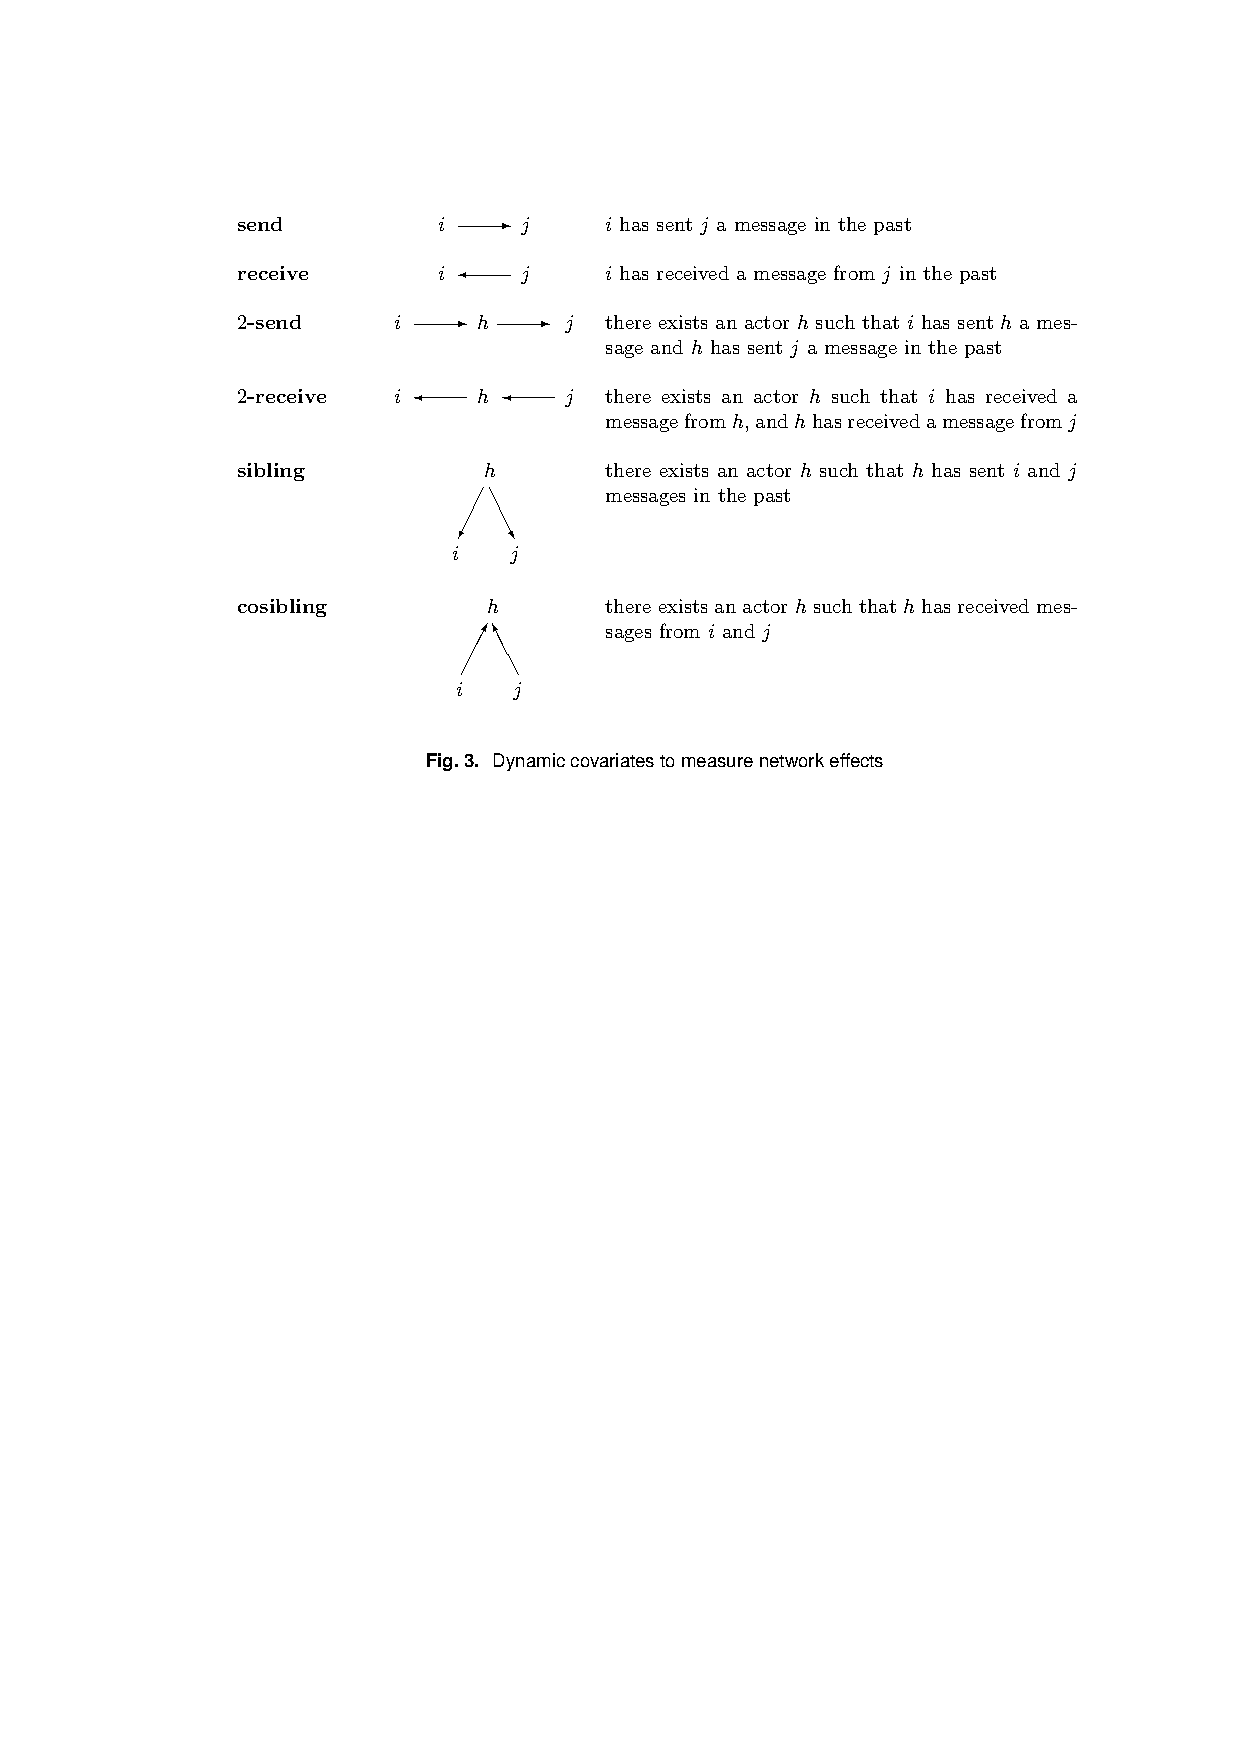
\includegraphics[width=0.6\textwidth]{PerryWolfe.pdf} 
	\label{fig:networkplot}
\end{figure}
By examining the estimates in Table 2 and their corresponding interpretaiton, it seems that there exist significant differences in the effect of some dynamic network covariates, especially dyadic effects (send and receive). In order to see these differences more clearly, we compared the posterior distribution using the boxplots in Figure 2. Now, it is more apparent that the intercept and dyadic effects are different across the interaction patterns. Specifically, IP5 seems to be highly dependent on the history of dyadic interactions; that is, whether the sender had sent to or received from the receiver strongly affects the rate of their interactions.
\begin{figure}[ht]
	\centering
	\includegraphics[width=0.88\textwidth]{boxplot2.pdf} 
	\caption{Posterior distribution of  $\boldsymbol{\beta}^{(c)}$ for Vance county emails}
	\label{fig:Vanceboxplot}
\end{figure}
\newline Next, we scrutinize the topic-word distributions corresponding to each interaction patterns in Table 3. Unlike $\boldsymbol{\beta}$, there is no distinctive difference in the topic distributions $\mathcal{Z}$, given the assignment of interaction patterns to the documents $\mathcal{C}$. The top three topics given the interaction patterns are quite overlapping, possibly because the unconditional distribution of topics reveal that Topic 2, 1, 5, 6, and 7 dominate the whole topic-word assignments, with the probabilities of these top five topics sum up to 0.533. Moreover, the actual words are not significantly different, having several words like `director', `phones', `church', `street', or `henderson' (county seat of Vance county) appeared repetitively across the topics as well as interaction patterns.
\footnotesize
\begin{comment}
\begin{table}[ht]
	\centering
	\begin{tabular}{|c|cccccccccc|} 
		\hline
		\textbf{Topic} & 2 &   1  &    5   & 6  &7    &15 &18    & 16   &11 &  12\\
		\hline
			\textbf{\#emails} & 958 & 843 & 783 & 742 & 61& 463 & 461 & 451 & 447&356\\
			\textbf{Prob.} & 0.128& 0.113& 0.105& 0.099&0.088&0.062&0.062& 0.060& 0.059&0.048\\
		\hline
	    	\textbf{Topic} &    17      &     8 &          3   & 9 &14&4  & 13 & 10 & 20 & 19\\\hline
		\textbf{\#emails} & 339& 325& 173& 98 & 91&78& 70&58 & 44&31\\	\textbf{Prob.}	& 0.045& 0.043&0.023& 0.013&0.012& 0.010&0.009&0.008& 0.006& 0.004\\ 
		\hline
	\end{tabular}
	\caption {Summary of posterior estimates of $\boldsymbol{\beta}^{(c)}$ for Vance county emails}
	\label{table:Vancetopic}
\end{table}
\end{comment}
\begin{table}[ht]
		\centering
\begin{tabular}{|l|l||l|l||l|l||l|l||l|l|}
	\hline
	\multicolumn{2}{|l||}{\textbf{IP1} (61 emails)}&\multicolumn{2}{l||}{\textbf{IP2} (38 emails)}&\multicolumn{2}{l||}{\textbf{IP3} (57 emails)}&\multicolumn{2}{l||}{\textbf{IP4} (56 emails)}&\multicolumn{2}{l|}{\textbf{IP5} (57 emails)}\\
	\hline\hline
	Topic 1&0.141&Topic 2&0.143&Topic 1 &0.151 & Topic 6 & 0.123 & Topic 2& 0.186 \\
	\hline
\scriptsize will&\scriptsize 0.0313&\scriptsize will&\scriptsize 0.0718&\scriptsize will&\scriptsize 0.0410&\scriptsize will&\scriptsize 0.0676&\scriptsize will&\scriptsize 0.0842\\
\scriptsize october&\scriptsize 0.0313&\scriptsize director&\scriptsize  0.0276&\scriptsize director&\scriptsize 0.0273&\scriptsize morning&\scriptsize 0.0338&\scriptsize director&\scriptsize 0.0330\\
\scriptsize description&\scriptsize  0.0223&\scriptsize system&\scriptsize 0.0276&\scriptsize description&\scriptsize 0.0239&\scriptsize electronic&\scriptsize 0.0338&\scriptsize opeartions&\scriptsize 0.0293\\
\scriptsize director&\scriptsize 0.0179&\scriptsize center&\scriptsize 0.0221&\scriptsize latest&\scriptsize 0.0239&\scriptsize church&\scriptsize 0.0270&\scriptsize phone&\scriptsize 0.0219\\
\scriptsize planning&\scriptsize 0.0179&\scriptsize directory&\scriptsize  0.0221&\scriptsize phones&\scriptsize 0.0205&\scriptsize suite&\scriptsize 0.0270&\scriptsize church&\scriptsize 0.0183\\
\scriptsize public&\scriptsize 0.0179&\scriptsize henderson&\scriptsize 0.0166&\scriptsize henderson&\scriptsize 0.0171&\scriptsize henderson&\scriptsize 0.0203&\scriptsize october&\scriptsize 0.0183\\
\scriptsize week&\scriptsize 0.0179&\scriptsize operations&\scriptsize 0.0166&\scriptsize attached&\scriptsize  0.0171&\scriptsize enp&\scriptsize 0.0203&\scriptsize street&\scriptsize 0.0147\\
\scriptsize henderson&\scriptsize 0.0134&\scriptsize suite&\scriptsize 0.0166&\scriptsize suite&\scriptsize 0.0137&\scriptsize hereto&\scriptsize  0.0203&\scriptsize development&\scriptsize  0.0147\\
\scriptsize phone&\scriptsize 0.0134&\scriptsize meeting&\scriptsize 0.0166&\scriptsize office&\scriptsize 0.0137&\scriptsize description&\scriptsize 0.0135&\scriptsize center&\scriptsize  0.0147\\
\scriptsize development&\scriptsize 0.0134&\scriptsize phone&\scriptsize  0.0166&\scriptsize cem&\scriptsize 0.0137&\scriptsize street&\scriptsize 0.0135&\scriptsize system&\scriptsize 0.0147\\
	\hline\hline
	Topic 2&0.134&Topic 17&0.115&Topic 5 &0.130& Topic 2 & 0.105 & Topic 7 & 0.137 \\
	\hline
	\scriptsize will&\scriptsize 0.0657&\scriptsize will&\scriptsize 0.0342&\scriptsize will&\scriptsize 0.0873&\scriptsize operations&\scriptsize 0.0476&\scriptsize will&\scriptsize 0.0448\\
	\scriptsize director&\scriptsize0.0329&\scriptsize week&\scriptsize 0.0342&\scriptsize street&\scriptsize 0.0278&\scriptsize director&\scriptsize 0.0397&\scriptsize jail &\scriptsize  0.0299\\
	\scriptsize phones&\scriptsize 0.0282&\scriptsize street&\scriptsize 0.0274&\scriptsize operations&\scriptsize 0.0278&\scriptsize suite&\scriptsize 0.0317&\scriptsize description&\scriptsize 0.0199\\
	\scriptsize department&\scriptsize 0.0235&\scriptsize message&\scriptsize  0.0274&\scriptsize church&\scriptsize 0.0238&\scriptsize message&\scriptsize 0.0317&\scriptsize emergency&\scriptsize 0.0199\\
	\scriptsize heads&\scriptsize 0.0235&\scriptsize church&\scriptsize 0.0205&\scriptsize description&\scriptsize 0.0198&\scriptsize street&\scriptsize 0.0238&\scriptsize center&\scriptsize  0.0199\\
	\scriptsize review&\scriptsize 0.0188&\scriptsize time&\scriptsize 0.0205&\scriptsize phone&\scriptsize 0.0198&\scriptsize planning&\scriptsize 0.0238&\scriptsize director&\scriptsize 0.0149\\
	\scriptsize october&\scriptsize 0.0188&\scriptsize lines&\scriptsize 0.0205&\scriptsize system&\scriptsize0.0198&\scriptsize  will&\scriptsize 0.0238&\scriptsize henderson&\scriptsize 0.0149\\
	\scriptsize system&\scriptsize 0.0188&\scriptsize operations&\scriptsize 0.0137&\scriptsize phones&\scriptsize0.0198&\scriptsize emergency&\scriptsize 0.0238&\scriptsize suite&\scriptsize 0.0149\\
	\scriptsize extension&\scriptsize 0.0188&\scriptsize meeting&\scriptsize 0.0137&\scriptsize  extension&\scriptsize0.0198&\scriptsize office&\scriptsize 0.0238&\scriptsize phone&\scriptsize 0.0149\\
	\scriptsize description&\scriptsize 0.0141&\scriptsize system&\scriptsize 0.0137&\scriptsize center&\scriptsize0.0159&\scriptsize today&\scriptsize 0.0238&\scriptsize office&\scriptsize 0.0149\\
	\hline\hline
	Topic 6&0.102&Topic 5&0.107&Topic 6&0.116& Topic 16 & 0.100& Topic 5&0.107\\
	\hline
	\scriptsize will&\scriptsize 0.0432&\scriptsize will&\scriptsize0.0889&\scriptsize will&\scriptsize 0.0982&\scriptsize message&\scriptsize 0.0417&\scriptsize street&\scriptsize 0.0446\\
	\scriptsize director&\scriptsize 0.0370&\scriptsize street&\scriptsize 0.0222&\scriptsize fax&\scriptsize0.0223&\scriptsize will&\scriptsize 0.0333&\scriptsize operations&\scriptsize 0.0255\\
	\scriptsize street&\scriptsize 0.0247&\scriptsize system&\scriptsize  0.0222&\scriptsize henderson&\scriptsize 0.0179&\scriptsize church&\scriptsize 0.0250&\scriptsize meeting&\scriptsize 0.0255\\
	\scriptsize electronic&\scriptsize 0.0247&\scriptsize questions&\scriptsize 0.0222&\scriptsize system&\scriptsize 0.0179&\scriptsize operations&\scriptsize 0.0250&\scriptsize folks&\scriptsize 0.0255\\
	\scriptsize heads&\scriptsize 0.0247&\scriptsize department&\scriptsize 0.0222&\scriptsize copies&\scriptsize 0.0179&\scriptsize electronic&\scriptsize 0.0250&\scriptsize coming&\scriptsize 0.0255\\
	\scriptsize fax&\scriptsize 0.0185&\scriptsize chapter&\scriptsize 0.0222&\scriptsize description&\scriptsize 0.0134&\scriptsize coming&\scriptsize 0.0250&\scriptsize henderson&\scriptsize  0.0191\\
	\scriptsize church&\scriptsize 0.0185&\scriptsize phones&\scriptsize 0.0222&\scriptsize church&\scriptsize  0.0134&\scriptsize latest&\scriptsize 0.0250&\scriptsize planning&\scriptsize 0.0191\\
	\scriptsize instructions&\scriptsize 0.0185&\scriptsize cutting&\scriptsize 0.0222&\scriptsize meeting&\scriptsize  0.0134&\scriptsize director&\scriptsize 0.0167&\scriptsize will&\scriptsize 0.0191\\
	\scriptsize time&\scriptsize 0.0185&\scriptsize director&\scriptsize 0.0148&\scriptsize heads&\scriptsize  0.0134&\scriptsize henderson&\scriptsize 0.0167&\scriptsize emergency&\scriptsize 0.0191\\
	\scriptsize message&\scriptsize 0.0185&\scriptsize henderson&\scriptsize 0.0148&\scriptsize sure&\scriptsize  0.0134&\scriptsize street&\scriptsize 0.0167&\scriptsize system&\scriptsize 0.0191\\
	\hline
\end{tabular}
	 		\caption {Summary of MCMC sampling results for Vance county emails. Each interaction pattern is shown with the top 3 topics and 10 words with the highest probability conditioned on that topic.}
	 		\label{table:Vancewords}
	 		\end{table}
\normalsize
\newline
Although Vance county email data did not display distinctive idiosyncrasy across the interaction patterns and their corresponding topic assignments, it is not surprising because Vance county is a small county (land area: 253.52 sq. mi and population: 44,998), and our exploratory data analysis did not find any significant change in the email exchanges of department managers during the period of hurricand Sandy. Yet, it is definitely worthwhile to further look at this in terms of showing the applicability of interaction-partitioned topic model (IPTM), in case of email data. In the next section, we apply the same method to another corpus, Dare county email data, in hope of finding more interesting results and also comparing the outcomes between the two counties.
\clearpage
\subsection{Dare county email data}
Application to Dare county email data was conducted in the exactly same manner as previous section. However, the size of Dare county data is much larger than that of Vance county data; that is, Dare county data contains 4,845 emails between 27 actors, including 2,907 vocabulary in total, after post-processing as before (i.e. multicast and word count $>$ 0).   Considering the huge expected computation time, we specified smaller number of topics, $K=10$, and smaller number of interaction patterns, $C=3$. Except those, all other parameters such as Dirichlet priors or MCMC parameters were identically specified as Section 4.1.
\footnotesize
\begin{table}[ht]
	\centering
	\begin{tabular}{|c|c|c|c|c|c|} 
		\hline
		& \textbf{IP1} & \textbf{IP2} &\textbf{IP3}&\textbf{IP4}&\textbf{IP5}\\
		\hline
		intercept &0.900 & -0.451& -0.795& 0.259&-0.856
		\\
		send&  0.409&-0.536& 2.755&  0.459& 1.972\\
		receive& 0.077&-0.616& 1.125&-0.185&0.721\\
		2-send&0.194&-1.201&0.062&-0.264&-0.997\\
		2-receive&-1.823&-0.411& -1.026& -1.203&0.873\\
		sibling&-0.678&0.981&  0.638&0.302&-0.403\\
		cosibling&-0.344&-1.402&-1.753& -1.333& -1.141\\
		\hline
	\end{tabular}
	\caption {Summary of posterior $\boldsymbol{\beta}^{(c)}$ estimates for Vance county emails}
	\label{table:AlexanderMCMC}
\end{table}
\begin{figure}[ht]
	\centering
	\includegraphics[width=0.74\textwidth]{boxplot2.pdf} 
	\caption{Posterior distribution of  $\boldsymbol{\beta}^{(c)}$ for Vance county emails}
	\label{fig:boxplot}
\end{figure}
\begin{table}[ht]
	\centering
	\begin{tabular}{|l|l||l|l||l|l||l|l||l|l|}
		\hline
		\multicolumn{2}{|l||}{\textbf{IP1} (56 emails)}&\multicolumn{2}{l||}{\textbf{IP2} (47 emails)}&\multicolumn{2}{l||}{\textbf{IP3} (69 emails)}&\multicolumn{2}{l||}{\textbf{IP4} (32 emails)}&\multicolumn{2}{l|}{\textbf{IP5} (65 emails)}\\
		\hline\hline
		Topic 15&0.212&Topic 18&0.181&Topic 9 &0.218 & Topic 14 & 0.302 & Topic 1 & 0.215 \\
		\hline
		\scriptsize operations&\scriptsize 0.0563&\scriptsize phone&\scriptsize 0.0395&\scriptsize electronic&\scriptsize 0.0789&\scriptsize will&\scriptsize 0.1250&\scriptsize will&\scriptsize 0.0523\\
		\scriptsize center&\scriptsize 0.0387&\scriptsize development&\scriptsize  0.0395&\scriptsize heads&\scriptsize 0.0366&\scriptsize phones&\scriptsize 0.0724&\scriptsize directory&\scriptsize 0.0494\\
		\scriptsize office&\scriptsize  0.0352&\scriptsize henderson&\scriptsize 0.0316&\scriptsize ncgs&\scriptsize 0.0338&\scriptsize week&\scriptsize 0.0395&\scriptsize jail&\scriptsize 0.0465\\
		\scriptsize communications&\scriptsize 0.0317&\scriptsize planning&\scriptsize 0.0316&\scriptsize attachments&\scriptsize 0.0310&\scriptsize system&\scriptsize 0.0373&\scriptsize extension&\scriptsize 0.0436\\
		\scriptsize enp&\scriptsize 0.0317&\scriptsize description&\scriptsize  0.0277&\scriptsize review&\scriptsize 0.0282&\scriptsize cutting&\scriptsize 0.0307&\scriptsize will&\scriptsize 0.0262\\
		\scriptsize suite&\scriptsize 0.0282&\scriptsize fax&\scriptsize 0.0277&\scriptsize chapter&\scriptsize 0.0282&\scriptsize rest&\scriptsize 0.0307&\scriptsize attached&\scriptsize 0.0262\\
		\scriptsize emergency&\scriptsize 0.0282&\scriptsize suite&\scriptsize 0.0237&\scriptsize pursuant&\scriptsize 0.0254&\scriptsize october&\scriptsize 0.0285&\scriptsize folks&\scriptsize 0.0262\\
		\scriptsize henderson&\scriptsize 0.0563&\scriptsize e-mail&\scriptsize 0.0237&\scriptsize department&\scriptsize 0.0225&\scriptsize provided&\scriptsize 0.0285&\scriptsize technology&\scriptsize 0.0262\\
		\scriptsize street&\scriptsize 0.0246&\scriptsize attached&\scriptsize 0.0237&\scriptsize tomorrow&\scriptsize 0.0225&\scriptsize department&\scriptsize 0.0241&\scriptsize excel&\scriptsize 0.0262\\
		\scriptsize director&\scriptsize 0.0211&\scriptsize director&\scriptsize  0.0198&\scriptsize time&\scriptsize 0.0197&\scriptsize phone&\scriptsize 0.0219&\scriptsize director&\scriptsize0.0233\\
		\hline\hline
		Topic 4&0.208&Topic 19&0.171&Topic 7 &0.208& Topic 12 & 0.298 & Topic 16 & 0.214 \\
		\hline
		\scriptsize emergency&\scriptsize 0.0466&\scriptsize description&\scriptsize 0.0546&\scriptsize message&\scriptsize 0.0531&\scriptsize will&\scriptsize 0.1064&\scriptsize will&\scriptsize 0.1023\\
		\scriptsize suite&\scriptsize0.0430&\scriptsize henderson&\scriptsize 0.0336&\scriptsize request&\scriptsize 0.0501&\scriptsize phones&\scriptsize 0.0643&\scriptsize extension&\scriptsize  0.0409\\
		\scriptsize director&\scriptsize 0.0358&\scriptsize director&\scriptsize 0.0252&\scriptsize electronic&\scriptsize 0.0442&\scriptsize october&\scriptsize 0.0377&\scriptsize folks&\scriptsize 0.0322\\
		\scriptsize fax&\scriptsize 0.0323&\scriptsize street&\scriptsize  0.0252&\scriptsize time&\scriptsize 0.0295&\scriptsize training&\scriptsize 0.0377&\scriptsize directory&\scriptsize 0.0292\\
		\scriptsize operations&\scriptsize 0.0323&\scriptsize church&\scriptsize 0.0210&\scriptsize review&\scriptsize 0.0295&\scriptsize department&\scriptsize 0.0310&\scriptsize call&\scriptsize 0.0263\\
		\scriptsize office&\scriptsize 0.0287&\scriptsize phone&\scriptsize 0.0210&\scriptsize department&\scriptsize 0.0295&\scriptsize provided&\scriptsize 0.0310&\scriptsize latest&\scriptsize 0.0263\\
		\scriptsize cem&\scriptsize 0.0287&\scriptsize goldvance...&\scriptsize 0.0210&\scriptsize response&\scriptsize0.0265&\scriptsize  system&\scriptsize 0.0288&\scriptsize cutover&\scriptsize 0.0205\\
		\scriptsize henderson&\scriptsize 0.0215&\scriptsize fax&\scriptsize 0.0168&\scriptsize manager&\scriptsize 0.0236&\scriptsize week&\scriptsize 0.0288&\scriptsize number&\scriptsize  0.0205\\
		\scriptsize will&\scriptsize 0.0179&\scriptsize suite&\scriptsize 0.0168&\scriptsize director&\scriptsize 0.0236&\scriptsize cutting&\scriptsize 0.0266&\scriptsize henderson&\scriptsize 0.0175\\
		\scriptsize phone&\scriptsize 0.0143&\scriptsize project&\scriptsize 0.0168&\scriptsize public&\scriptsize0.0206&\scriptsize day&\scriptsize 0.0222&\scriptsize advised&\scriptsize 0.0175\\
		\hline\hline
		Topic 8&0.199&Topic 3&0.161&Topic 11 &0.204& Topic 17 & 0.271& Topic 2&0.202\\
		\hline
		\scriptsize operations&\scriptsize 0.0489&\scriptsize description&\scriptsize0.0446&\scriptsize department&\scriptsize 0.0631&\scriptsize will&\scriptsize 0.0854&\scriptsize will&\scriptsize 0.1022\\
		\scriptsize emergency&\scriptsize 0.0489&\scriptsize e-mail&\scriptsize 0.0357&\scriptsize message&\scriptsize0.0511&\scriptsize phone&\scriptsize 0.0390&\scriptsize latest&\scriptsize 0.0310\\
		\scriptsize director&\scriptsize 0.0338&\scriptsize developement&\scriptsize  0.0313&\scriptsize records&\scriptsize 0.0420&\scriptsize october&\scriptsize 0.0390&\scriptsize extension&\scriptsize 0.0279\\
		\scriptsize henderson&\scriptsize 0.0338&\scriptsize director&\scriptsize 0.0268&\scriptsize heads&\scriptsize 0.0360&\scriptsize week&\scriptsize 0.0341&\scriptsize jail&\scriptsize 0.0279\\
		\scriptsize fax&\scriptsize 0.0338&\scriptsize goldvance...&\scriptsize 0.0268&\scriptsize will&\scriptsize 0.0330&\scriptsize phones&\scriptsize 0.0268&\scriptsize updated&\scriptsize 0.0248\\
		\scriptsize street&\scriptsize 0.0301&\scriptsize church&\scriptsize 0.0223&\scriptsize electronic&\scriptsize 0.0330&\scriptsize folks&\scriptsize 0.0268&\scriptsize director&\scriptsize  0.0217\\
		\scriptsize center&\scriptsize 0.0301&\scriptsize henderson&\scriptsize 0.0179&\scriptsize pursuant&\scriptsize 0.0330&\scriptsize rest&\scriptsize 0.0244&\scriptsize attached&\scriptsize 0.0217\\
		\scriptsize office&\scriptsize 0.0263&\scriptsize street&\scriptsize 0.0179&\scriptsize chapter&\scriptsize 0.0300&\scriptsize senior&\scriptsize 0.0244&\scriptsize coming&\scriptsize 0.0171\\
		\scriptsize church&\scriptsize 0.0188&\scriptsize phone&\scriptsize 0.0179&\scriptsize manager&\scriptsize 0.0270&\scriptsize system&\scriptsize 0.0220&\scriptsize henderson&\scriptsize 0.0163\\
		\scriptsize enp&\scriptsize 0.0188&\scriptsize semprius&\scriptsize 0.0179&\scriptsize response&\scriptsize 0.0240&\scriptsize directory&\scriptsize 0.0220&\scriptsize cutover&\scriptsize  0.0154\\
		\hline
	\end{tabular}
	\caption {Summary of MCMC sampling results for Vance county emails. Each interaction pattern is shown with the top 3 topics and words that have the highest probability conditioned on that topic.}
	\label{table:VanceMCMC}
\end{table}
\normalsize
\begin{comment}
\section{Preliminary Analysis}
Hurricane Sandy was the most destructive hurricane in 2012, which hit North Carolina on late October (October 28, Governor Bev Perdue declared a state of emergency in 24 western counties due to snow and strong winds). In our dataset, there are three counties which cover the date of Hurricane Sandy (October 22, 2012 – November 2, 2012), so we focus on the three counties, since the timestamp of email in this case is much more important than usual case without any disastrous event.
\subsection{Dare County}
\footnotesize
\begin{table}[ht]
	\centering
	\begin{tabular}{ |c|ccc|c| } 
		\hline 
		\textbf{Period} &\textbf{Before Sandy} & \textbf{During Sandy} & \textbf{After Sandy} & \textbf{Overall} \\ 	\hline
			\textbf{\# emails}& 1933 & 1563 & 1467 & 4963 \\ 
		\hline
	\end{tabular}
	\caption{ Summary of Dare county email data based on time period}
	\label{table:nullDare2}
\end{table}
\normalsize
Before Sandy ranges from 2012-09-01 to 2012-10-21 (7 weeks), During Sandy ranges from 2012-10-22 to 2012-11-02 (2 weeks), and After Sandy ranges from 2012-11-03 to 2012-11-30 (4 weeks).
\footnotesize
\begin{figure}[ht]
	\centering
	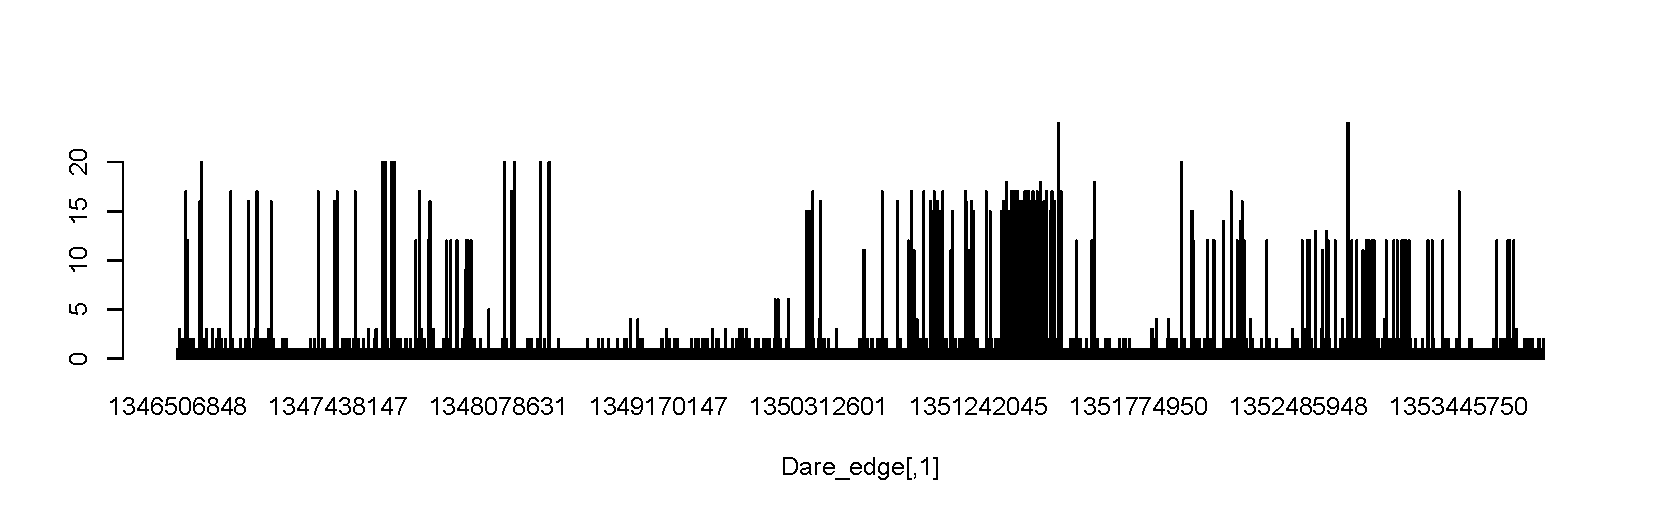
\includegraphics[width=1.1\textwidth]{DareEmails.pdf} 
	\caption{Frequency of Dare county emails from 2012-09-01 to 2012-11-30  }
	\label{fig:Emailplots}
\end{figure}
\begin{table}[ht]
	\centering
	\begin{tabular}{ |c|cc| } 
		\hline 
		\textbf{Time Interval} &\textbf{send} & \textbf{receive} \\ 	
		\hline  $[-\infty, t)$&  2.128, 2.659, 2.355, 2.919& 0.292, 0.257, 0.047, 0.110\\  $[t-30 m, t)$ &  0.262, -0.064, 0.782, 0.317 &2.087, 1.287 , 2.346, 1.870\\  $[t-2h, t-30m)$& 0.383, 0.157 , 0.024, -0.045 &0.553, 0.082, 0.794, 0.269\\ $[t-8h, t-2h)$ & 0.816, 0.054 , 0.077, 0.381 &-0.221, 0.048, 0.298, -0.012 \\ $[t-32h, t-8h)$& 0.085, 0.014,  0.228, 0.070 &0.101, 0.017, -0.033, 0.019\\ $[t-5.33d, t-32h)$&  0.103, 0.025, 0.092, 0.008 &-0.027, -0.016, -0.033, -0.009 \\ $[t-21.33d, t-5.33d)$  & 0.052, 0.000, 0.059, 0.010& 0.013, 0.030 , -0.016, 0.013\\ 
		$[-\infty, t-21.33d)$  & 0.052, 0.103, 0.027, 0.021  & 0.008, 0.000, 0.020, -0.005\\
		\hline
	\end{tabular}
	\caption {Estimated coefficients and approximate standard errors for dyadic effects of Dare county data (before Sandy, during Sandy, after Sandy, overall)}
	\label{table:nullDare}
\end{table}
\footnotesize
\begin{figure}[ht]
	\centering
	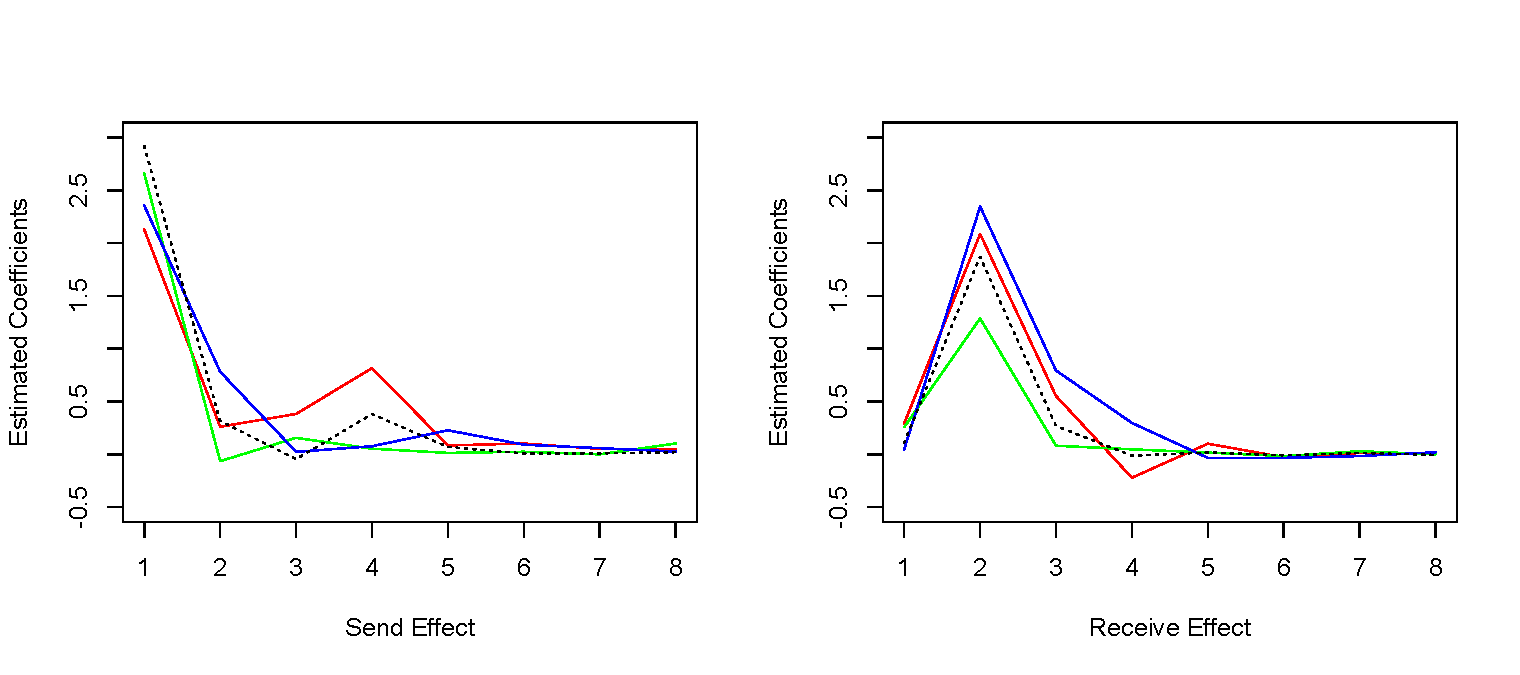
\includegraphics[width=1.1\textwidth]{Dareplot.pdf} 
	\caption{Comparison of Send (left) and Receive (right) effect based on periods in Table 1. (Red=Before, Green=During, Blue=After, and dot=Overall)}	\label{fig:Emailplo22t}
\end{figure}
\subsection{Lenoir County}
\footnotesize
\begin{table}[ht]
	\centering
	\begin{tabular}{ |c|ccc|c| } 
		\hline 
		\textbf{Period} &\textbf{Before Sandy} & \textbf{During Sandy} & \textbf{After Sandy} & \textbf{Overall} \\ 	\hline
		\textbf{\# emails}& 216 & 83 & 302 & 601 \\ 
		\hline
	\end{tabular}
	\caption{ Summary of Lenoir county email data based on time period}
	\label{table:nullDare22}
\end{table}
\normalsize
Before Sandy ranges from 2012-10-01 to 2012-10-21 (3 weeks), During Sandy ranges from 2012-10-22 to 2012-11-02 (2 weeks), and After Sandy ranges from 2012-11-03 to 2012-12-31 (8 weeks).
\footnotesize
\begin{figure}[ht]
	\centering
	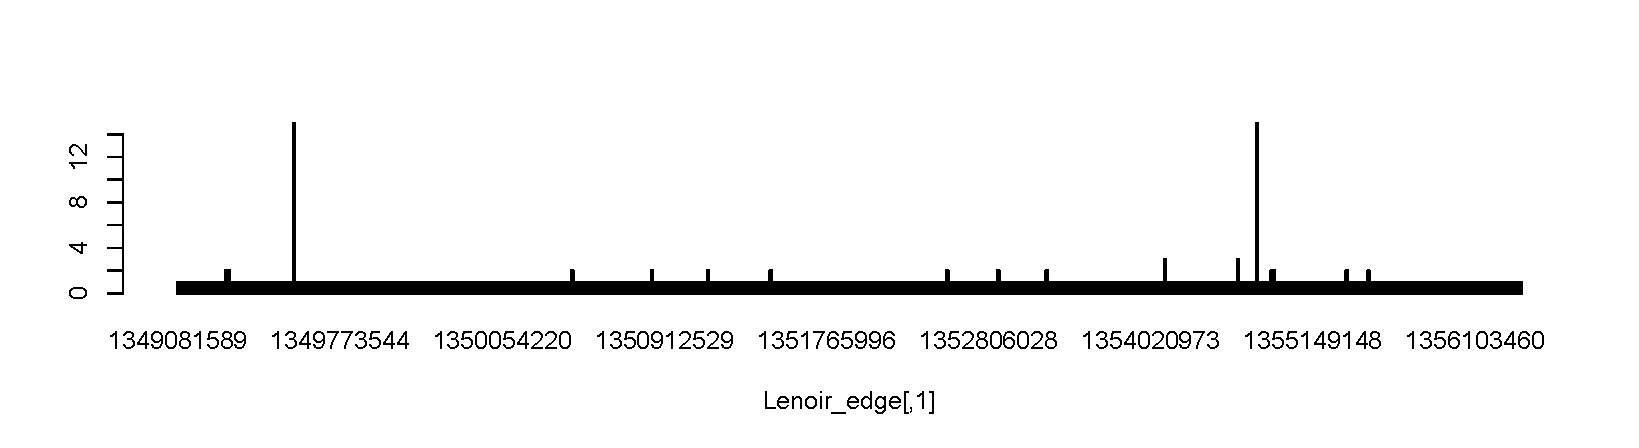
\includegraphics[width=1.1\textwidth]{LenoirEmails.pdf} 
	\caption{Frequency of Lenoir county emails from 2012-10-01 to 2012-12-31  }
	\label{fig:Emailplots32}
\end{figure}
\newpage
\subsection{Vance County}
\footnotesize
\footnotesize
\begin{table}[ht]
	\centering
	\begin{tabular}{ |c|ccc|c| } 
		\hline 
		\textbf{Period} &\textbf{Before Sandy} & \textbf{During Sandy} & \textbf{After Sandy} & \textbf{Overall} \\ 	\hline
		\textbf{\# emails}& 198& 18 & 55 & 271 \\ 
		\hline
	\end{tabular}
	\caption{ Summary of Vance county email data based on time period}
	\label{table:nullVance}
\end{table}
\normalsize
Before Sandy ranges from 2012-09-04 to 2012-10-21 (7 weeks), During Sandy ranges from 2012-10-22 to 2012-11-02 (2 weeks), and After Sandy ranges from 2012-11-03 to 2012-11-30  (4 weeks).
\footnotesize
\begin{figure}[ht]
	\centering
	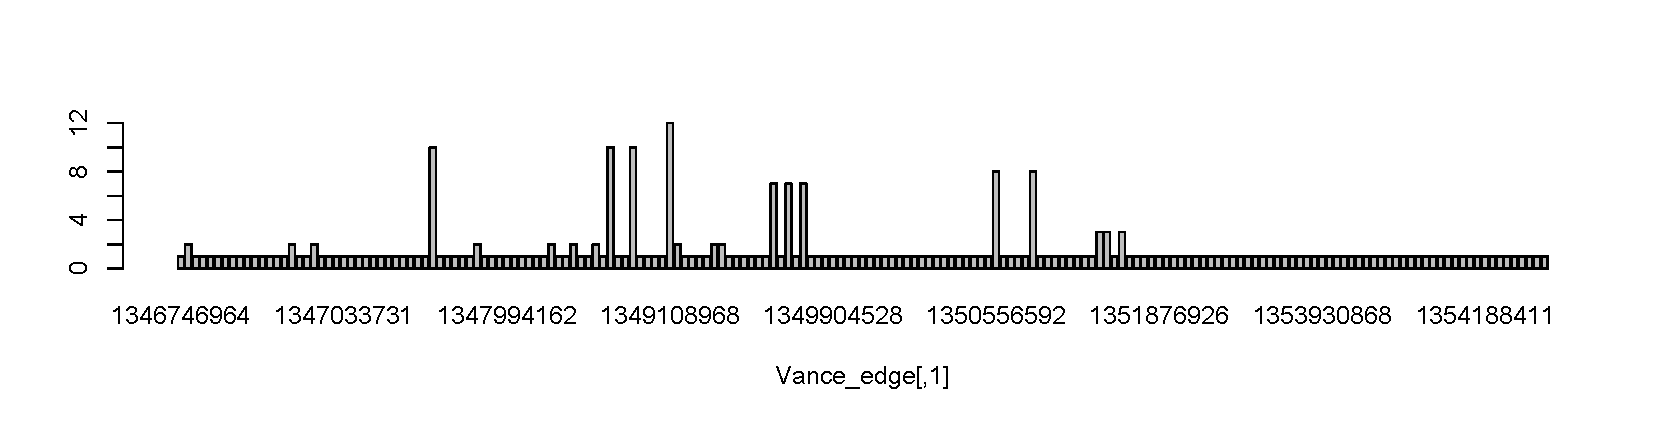
\includegraphics[width=1.1\textwidth]{VanceEmails.pdf} 
	\caption{Frequency of Vance county emails from 2012-09-04 to 2012-11-30  }
	\label{fig:Emailplots22}
\end{figure}
\end{comment}
\clearpage
\section*{APPENDIX}
\subsection*{APPENDIX A: Deriving the sampling equations for IPTM}
\begin{equation}
\begin{aligned}
& P(\Phi, \Theta, \mathcal{W}, \mathcal{Z}, \mathcal{C}, \mathcal{B}, \mathcal{N}| \mathcal{X}, \delta, \boldsymbol{n}, \alpha, \boldsymbol{m}, \boldsymbol{\gamma}, \boldsymbol{\eta}, \sigma^2) \\& 
=  P(\mathcal{W}, \mathcal{Z}, \mathcal{C}, \mathcal{B}, \mathcal{N}| \Phi, \Theta, \mathcal{X}, \boldsymbol{\gamma}, \boldsymbol{\eta}, \sigma^2) P(\Phi, \Theta |\delta, \boldsymbol{n}, \alpha, \boldsymbol{m})
\\&= P( \mathcal{W}| \mathcal{Z}, \Phi)P(\mathcal{Z}|\Theta)P(\mathcal{N}|\mathcal{C}, \mathcal{B}, \mathcal{X})P(\mathcal{B}|\mathcal{C}, \sigma^2)P(\Phi|\delta, \boldsymbol{n})P(\Theta|\mathcal{C}, \alpha, \boldsymbol{m})P(\mathcal{C}|\boldsymbol{\gamma})P(\boldsymbol{\gamma}|\boldsymbol{\eta})
\\&= \Big[\prod_{d=1}^{D}\prod_{m=1}^{M^{(d)}} P( w_m^{(d)}| \phi_{z_m^{(d)}})\Big]\times \Big[\prod_{d=1}^{D}\prod_{m=1}^{M^{(d)}} P( z_m^{(d)}| \boldsymbol{\theta}^{(c)})\Big]\times \Big[\prod_{d=1}^{D} P( \mathbf{N}^{(d)}(t^{(d)})| c^{(d)}, \boldsymbol{x}(t^{(d)}), \boldsymbol{\beta}^{(c)})\Big]  \\&\quad \quad \times\Big[\prod_{c=1}^{C} P( \boldsymbol{\beta}^{(c)}| \sigma^2)\Big]\times\Big[\prod_{k=1}^{K} P( \boldsymbol{\phi}^{(k)}| \delta, \boldsymbol{n})\Big]\times \Big[\prod_{c=1}^{C} P( \boldsymbol{\theta}^{(c)}|\alpha, \boldsymbol{m})\Big]\times \Big[\prod_{d=1}^{D} P(c^{(d)}|\boldsymbol{\gamma})\Big]  \times P(\boldsymbol{\gamma}|\boldsymbol{\eta})
\end{aligned}
\end{equation}
Since $P( \boldsymbol{\beta}^{(c)}| \sigma^2)$ is $\mbox{Normal}(\boldsymbol{0}, \sigma^2)$ and $P(\boldsymbol{\gamma}|\boldsymbol{\eta})$ is $\mbox{Dirichlet}(\boldsymbol{\eta})$, we can drop the two terms out and further rewrite the equation (20) as below:
\begin{equation}
\begin{aligned}
& \propto \Big[\prod_{d=1}^{D}\prod_{m=1}^{M^{(d)}} P( w_m^{(d)}| \phi_{z_m^{(d)}})\Big]\times \Big[\prod_{d=1}^{D}\prod_{m=1}^{M^{(d)}} P( z_m^{(d)}| \boldsymbol{\theta}^{(c)})\Big]\times \Big[\prod_{d=1}^{D} P( \mathbf{N}^{(d)}(t^{(d)})| c^{(d)}, \boldsymbol{x}(t^{(d)}), \boldsymbol{\beta}^{(c)})\Big]\\& \quad \quad  \times\Big[\prod_{k=1}^{K} P( \boldsymbol{\phi}^{(k)}| \delta, \boldsymbol{n})\Big] \times\Big[\prod_{c=1}^{C} P( \boldsymbol{\theta}^{(c)}|\alpha, \boldsymbol{m})\Big] \times\Big[\prod_{d=1}^{D} P(c^{(d)}|\boldsymbol{\gamma})\Big] \\&
= \Big[\prod_{d=1}^{D}\prod_{m=1}^{M^{(d)}} \phi_{w_m^{(d)}z_m^{(d)}}\Big]\times \Big[\prod_{d=1}^{D}\prod_{m=1}^{M^{(d)}} \boldsymbol{\theta}^{(c)}_{z_m^{(d)}}\Big]\times\Big[\prod_{d=1}^{D} \frac{\mbox{exp}\{\boldsymbol{\beta}^{(c)T}x_{t^{(d)}}(i^{(d)}, j^{(d)})\}}{\sum_{j\in \mathcal{A}^{(c)}} \mbox{exp}\{\boldsymbol{\beta}^{(c)T}x_{t^{(d)}}(i^{(d)}, j)\}}\Big]\\& \quad \quad \times \Big[\prod_{k=1}^{K} \Big(\frac{\Gamma(\sum_{w=1}^{W}\delta n_w)}{\prod_{w=1}^{W}\Gamma(\delta n_w)}\prod_{w=1}^{W}\phi_{wk}^{\delta n_w-1} \Big)\Big]\times \Big[\prod_{c=1}^{C} \Big(\frac{\Gamma(\sum_{k=1}^{K}\alpha m_k)}{\prod_{k=1}^{K}\Gamma(\alpha m_k)}\prod_{k=1}^{K}(\boldsymbol{\theta}^{(c)}_{k})^{\alpha m_k-1} \Big)\Big] \times\Big[\prod_{d=1}^{D} \gamma_{c}^{I(c^{(d)}=c)}\Big] \\&
=\Big[\frac{\Gamma(\sum_{w=1}^{W}\delta n_w)}{\prod_{w=1}^{W}\Gamma(\delta n_w)}\Big]^K \times \Big[\frac{\Gamma(\sum_{w=1}^{W}\delta n_w)}{\prod_{w=1}^{W}\Gamma(\delta n_w)}\Big]^C \times\Big[\prod_{d=1}^{D} \frac{\mbox{exp}\{\boldsymbol{\beta}^{(c)T}x_{t^{(d)}}(i^{(d)}, j^{(d)})\}}{\sum_{j\in \mathcal{A}^{(c)}} \mbox{exp}\{\boldsymbol{\beta}^{(c)T}x_{t^{(d)}}(i^{(d)}, j)\}}\Big]\\&\quad\quad\times\Big[\prod_{d=1}^{D}\gamma_{c^{(d)}}\Big]\times
\Big[\prod_{k=1}^{K}\prod_{w=1}^{W}\phi_{wk}^{M^{WK}_{wk}+\delta n_w-1}\Big]\times\Big[\prod_{c=1}^{C}\prod_{k=1}^{K}(\boldsymbol{\theta}^{(c)}_{k})^{M^{CK}_{ck}+\alpha m_k-1}\Big]
\end{aligned}
\end{equation}
where $M^{WK}_{wk}$ is the number of times the $w^{th}$ word in the vocabulary is assigned to topic $k$, and $M^{CK}_{ck}$ is the number of times topic k shows up given the interaction pattern $c$. By looking at the forms of the terms involving  $\Theta$ and $\Phi$ in Equation (21), we integrate out the random variables $\Theta$ and $\Phi$, making use of the fact that the Dirichlet distribution is a conjugate prior of multinomial distribution. Applying the well-known formula $\int\prod_{m=1}^{M}[x_m^{k_m-1}dx_m]=\frac{\prod_{m=1}^M\Gamma(k_m)}{\Gamma(\sum_{m=1}^Mk_m)}$ to (22), we have:
\begin{equation}
\begin{aligned}
&P(\mathcal{W}, \mathcal{Z}, \mathcal{C}, \mathcal{B}, \mathcal{N}| \mathcal{X}, \delta, \boldsymbol{n}, \alpha, \boldsymbol{m}, \boldsymbol{\gamma}, \boldsymbol{\eta}, \sigma^2)\\&=\mbox{Const.}\int_{\Theta}\int_{\Phi}\Big[\prod_{k=1}^{K}\prod_{w=1}^{W}\phi_{wk}^{M^{WK}_{wk}+\delta n_w-1}\Big]\Big[\prod_{c=1}^{C}\prod_{k=1}^{K}(\boldsymbol{\theta}^{(c)}_{k})^{M^{CK}_{ck}+\alpha m_k-1}\Big]d\Phi d\Theta
\\&=\mbox{Const.}\Big[\prod_{k=1}^{K}\int_{\phi_{:k}}\prod_{w=1}^{W}\phi_{wk}^{M^{WK}_{wk}+\delta n_w-1  }d\phi_{:k}\Big]\times\Big[\prod_{c=1}^{C}\int_{\theta_{:c}}\prod_{k=1}^{K}(\boldsymbol{\theta}^{(c)}_{k})^{M^{CK}_{ck}+\alpha m_k-1}d\theta_{:c}\Big]
\\&=\mbox{Const.}\Big[\prod_{k=1}^{K}\frac{\prod_{w=1}^W\Gamma(M_{wk}^{WK}+\delta n_w)}{\Gamma(\sum_{w=1}^WM_{wk}^{WK}+\delta )}\Big]\times\Big[\prod_{c=1}^{C}\frac{\prod_{k=1}^K\Gamma(M^{CK}_{ck}+\alpha m_k)}{\Gamma(\sum_{k=1}^KM^{CK}_{ck}+\alpha)}\Big].
\end{aligned}
\end{equation}
\subsection*{APPENDIX B: Computing conditional probability}
\begin{equation}
\begin{aligned}
& P(\boldsymbol{w}^{(d)}, \boldsymbol{z}^{(d)}|c^{(d)}=c, \mathcal{W}_{\backslash d}, \mathcal{Z}_{\backslash d}, \mathcal{C}_{\backslash d}, \delta, \boldsymbol{n}, \alpha, \boldsymbol{m}) \\& \propto \prod_{m=1}^{M^{(d)}}P(z^{(d)}_m=k, w^{(d)}_m=w| c^{(d)}=c, \mathcal{W}_{\backslash d, m}, \mathcal{Z}_{\backslash d,m}, \mathcal{C}_{\backslash d}, \delta, \boldsymbol{n}, \alpha, \boldsymbol{m})
\end{aligned}
\end{equation} 
To obtain the Gibbs sampling equation, we need to obtain an expression for $P(z^{(d)}_m=k,  w^{(d)}_m=w, c^{(d)}=c|\mathcal{W}_{\backslash d}, \mathcal{Z}_{\backslash d}, \mathcal{C}_{\backslash d}, \delta, \boldsymbol{n}, \alpha, \boldsymbol{m})$,
 From Bayes' theorem and Gamma identity $\Gamma(k+1)=k\Gamma(k)$,
\begin{equation}
\begin{aligned}
& P(z^{(d)}_m=k, w^{(d)}_m=w, c^{(d)}=c|\mathcal{W}_{\backslash d, m}, \mathcal{Z}_{\backslash d,m}, \mathcal{C}_{\backslash d}, \delta, \boldsymbol{n}, \alpha, \boldsymbol{m}) \\& \propto 
\frac{P(\mathcal{W}, \mathcal{Z}, \mathcal{C}|\delta, \boldsymbol{n}, \alpha, \boldsymbol{m})}{P(\mathcal{W}_{\backslash d, m}, \mathcal{Z}_{\backslash d, m}, \mathcal{C}|\delta, \boldsymbol{n}, \alpha, \boldsymbol{m})}\\& \propto \frac{\prod_{k=1}^{K}\frac{\prod_{w=1}^W\Gamma(M_{wk}^{WK}+\delta n_w)}{\Gamma(\sum_{w=1}^WM_{wk}^{WK}+\delta )}\times\prod_{c=1}^{C}\frac{\prod_{k=1}^K\Gamma(M^{CK}_{ck}+\alpha m_k)}{\Gamma(\sum_{k=1}^KM^{CK}_{ck}+\alpha)}}{\prod_{k=1}^{K}\frac{\prod_{w=1}^W\Gamma(M_{wk, \backslash d, m}^{WK}+\delta n_w)}{\Gamma(\sum_{w=1}^WM_{wk, \backslash d, m}^{WK}+\delta )}\times\prod_{c=1}^{C}\frac{\prod_{k=1}^K\Gamma(M^{CK}_{ck, \backslash d, m}+\alpha m_k)}{\Gamma(\sum_{k=1}^KM^{CK}_{ck, \backslash d, m}+\alpha)}}\\ & \propto 
\frac{M_{wk, \backslash d, m}^{WK}+\delta n_w}{\sum_{w=1}^WM_{wk,  \backslash d, m}^{WK}+\delta}\times\frac{M^{CK}_{ck, \backslash d, m}+\alpha m_k}{\sum_{k=1}^KM^{CK}_{ck, \backslash d, m}+\alpha}
\end{aligned}
\end{equation}
Then, the conditional probability that a novel word generated in the document of interaction pattern $c^{(d)}=c$  would be assigned to topic $z_m^{(d)}=k$ is obtained by:
 \begin{equation}
 \begin{aligned}
 &P(z^{(d)}_m=k|w^{(d)}_m=w, c^{(d)}=c, \mathcal{W}_{\backslash d, m}, \mathcal{Z}_{\backslash d,m}, \mathcal{C}_{\backslash d}, \delta, \boldsymbol{n}, \alpha, \boldsymbol{m}) \\& \propto
 \frac{M^{CK}_{ck, \backslash d, m}+\alpha m_k}{\sum_{k=1}^KM^{CK}_{ck, \backslash d, m}+\alpha}
 \end{aligned}
 \end{equation}
In addition, the conditional probability that a new word generated in the document would be $w_m^{(d)}=w$, given that it is generated from topic $z_m^{(d)}=k$ is obtained by:
\begin{equation}
\begin{aligned}
& P(w^{(d)}_m=w|z^{(d)}_m=k, c^{(d)}=c, \mathcal{W}_{\backslash d, m}, \mathcal{Z}_{\backslash d,m}, \mathcal{C}_{\backslash d}, \delta, \boldsymbol{n}, \alpha, \boldsymbol{m}) \\& \propto 
\frac{M_{wk, \backslash d, m}^{WK}+\delta n_w}{\sum_{w=1}^WM_{wk, \backslash d, m}^{WK}+\delta}
\end{aligned} 
 \end{equation}
 \subsection*{APPENDIX C: MCMC Diagnostics for Vance county emails}
 \begin{figure}[ht]
 	\centering
 	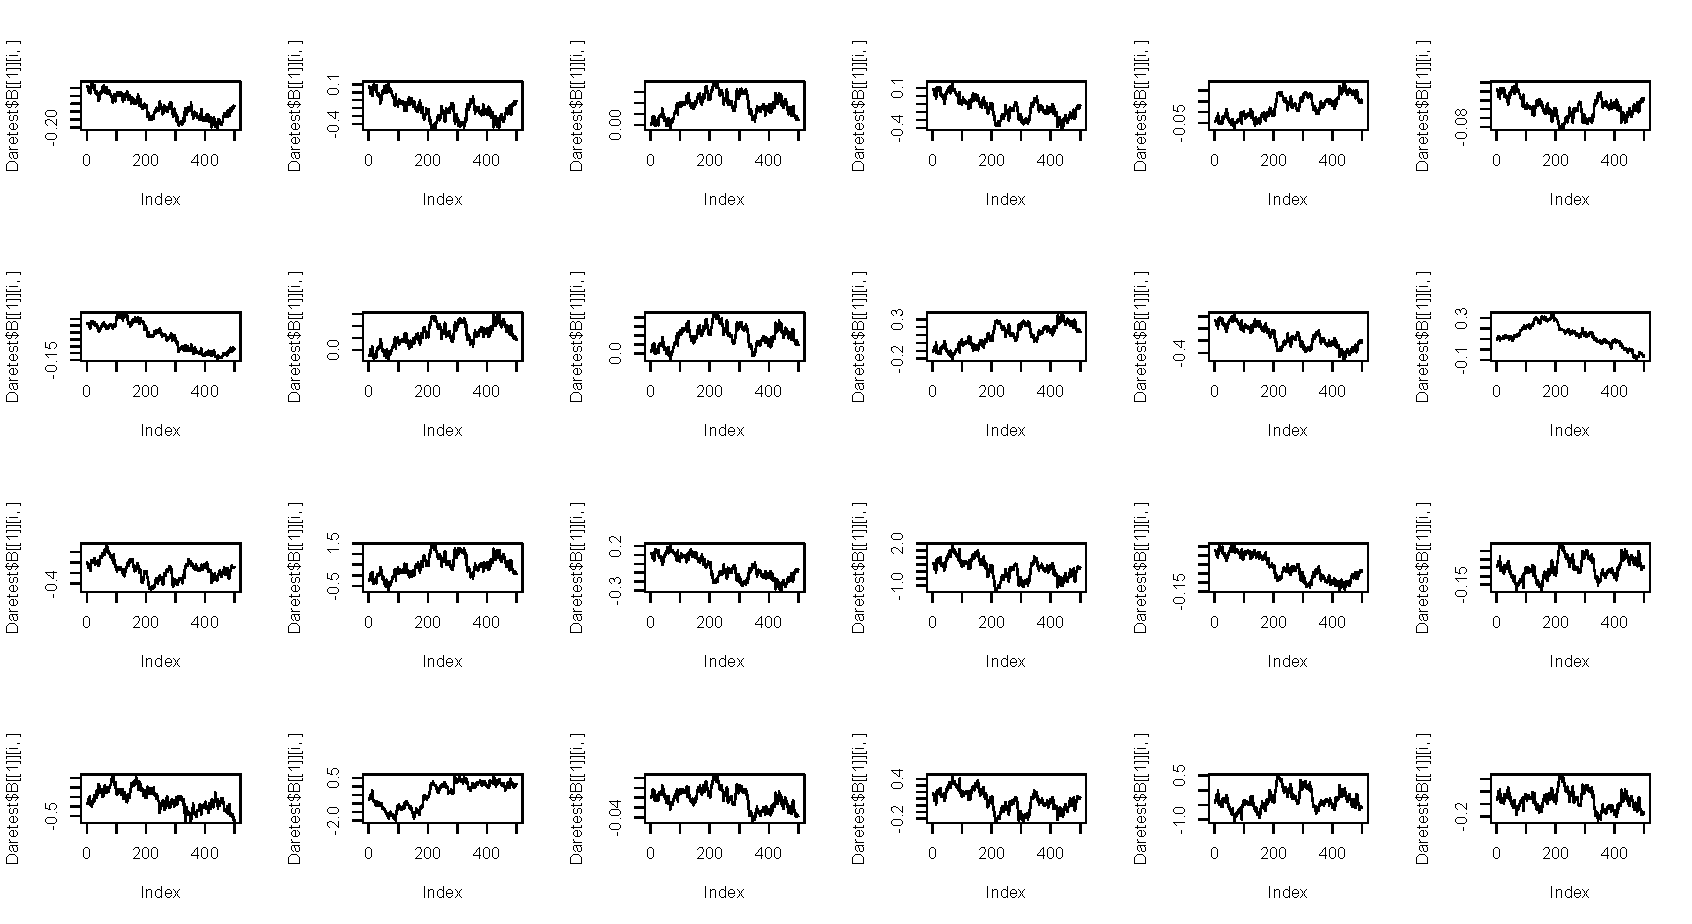
\includegraphics[width=1\textwidth]{IP1.pdf} 
 		\caption{Traceplots and density plots of $\boldsymbol{\beta}^{(1)}$}
 	\label{fig:IP1}
 	 \end{figure}
 	  \begin{figure}[ht]
 	  	\centering
 	 	\includegraphics[width=1\textwidth]{IP5.pdf} 
 		 		 		\label{fig:IP5}
 			\caption{Traceplots and density plots of $\boldsymbol{\beta}^{(5)}$}
 	 \end{figure}
\bibliographystyle{apalike}
\bibliography{BominBib}

\end{document}